\chapter{DMN: Detección de ataques morphing\label{ch:morphing}}

% Sin embargo, el enfoque desarrollado por los autores se divide en dos objetivos. El primer objetivo consiste en desentrañar la identidad criminal. El segundo objetivo se basa en comparar la imagen obtenida en la etapa anterior con la imagen \gls{vivo} obtenida en la puerta \GLS{ABC}. Por lo tanto, los autores pueden concluir si el ataque de morphing ocurrió o no. Además, el proceso de \textit{\gls{de-morphing}} de \textit{Peng et al.} se basa en una \GLS{GAN}, pero el enfoque presentado se basa en una arquitectura de auto-codificador. En cuanto a la \GLS{DMN}, otro punto clave es que ninguno de los enfoques considera las imágenes de impresión y escaneo en sus estudios. Finalmente, los trabajos de \textit{Peng} y \textit{Ferrara} toman las imágenes para su base de datos en un ambiente controlado. Sin embargo, en este trabajo de investigación, se utilizan $1170$ imágenes tomadas en el sistema de control de embarque automatizado \glspl{e-gate}.

La idea de fusionar dos imágenes para conseguir un efecto visual sorprendente es algo muy antiguo. Desde las \textit{tabula scalatas} (tablas escaladas (fig. \ref{fig:tabula_scalata})) del renacimiento hasta las cámaras oscuras con disolución de imágenes (Dissolving Views) del siglo XIX (var Fig. \ref{fig:disolving_views}). Pero fue con la imagen digital cuando se consigue que estos efectos sean realmente convincentes. A finales de los años $80$, principios de los $90$, muchas producciones visuales, como películas, anuncios o vídeos musicales (ver Fig. \ref{fig:first_morphing_samples}) comenzaron a hacer uso de técnicas de \textit{\gls{morphing} digital} y aparecieron los primeros estudios científicos sobre el tema \cite{lee1998polymorph} \cite{ucicr1992feature}.

\begin{figure}[h!]
    \centering
    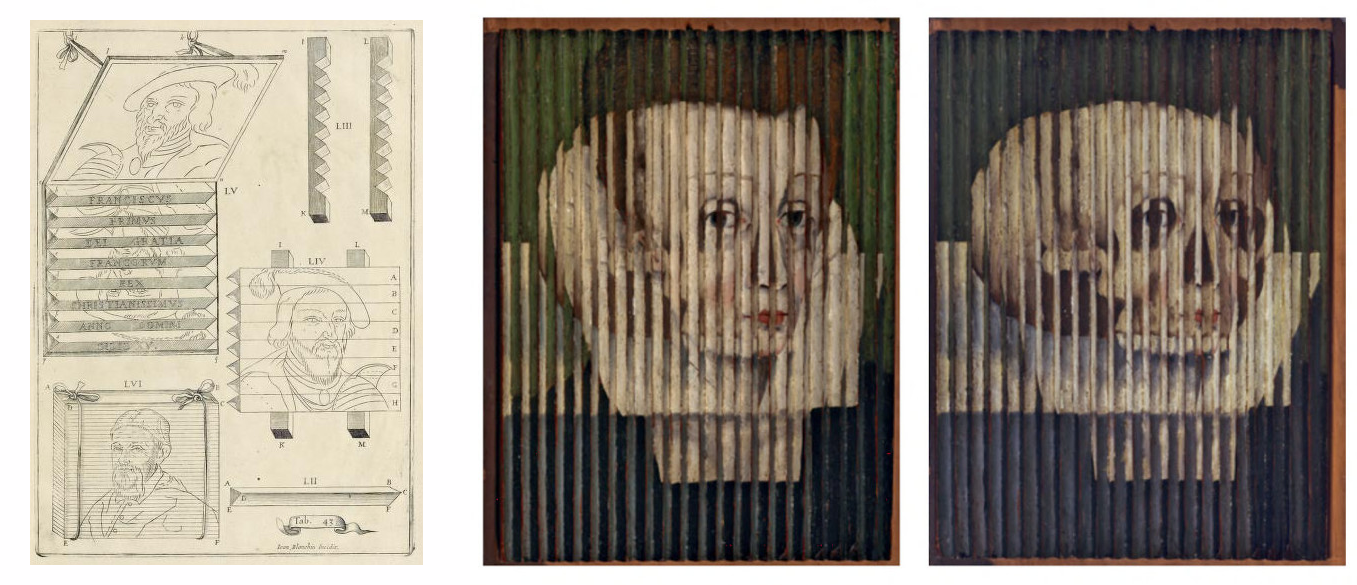
\includegraphics[width=0.6\textwidth]{ch-sistemasABC/images/ch-morphing/old/tabula_scalata.png}
    \caption{\textit{Tabula Scalata} \cite{rodrigo2011anamorfosis}.}
    \label{fig:tabula_scalata}
\end{figure}

\begin{figure}[h!]
    \centering
    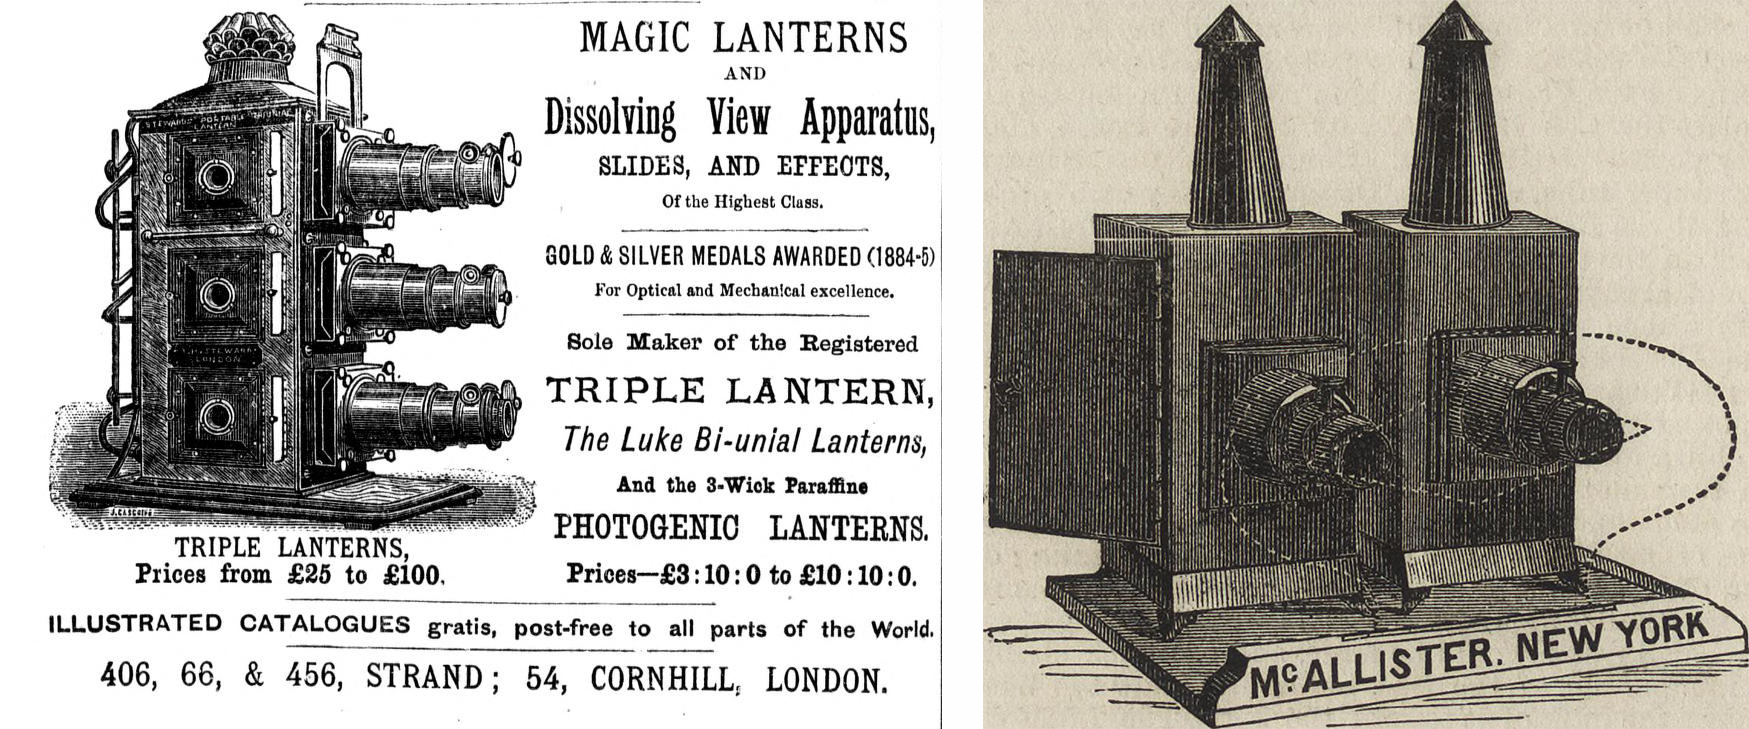
\includegraphics[width=0.6\textwidth]{ch-sistemasABC/images/ch-morphing/old/DisolvingViews.png}
    \caption{Linternas mágicas con \textit{dissolving view} \cite{higson2016dissolving}.}
    \label{fig:disolving_views}
\end{figure}

\begin{figure}[t!]
     \centering
    \begin{subfigure}[b]{0.6\textwidth}
        \centering
        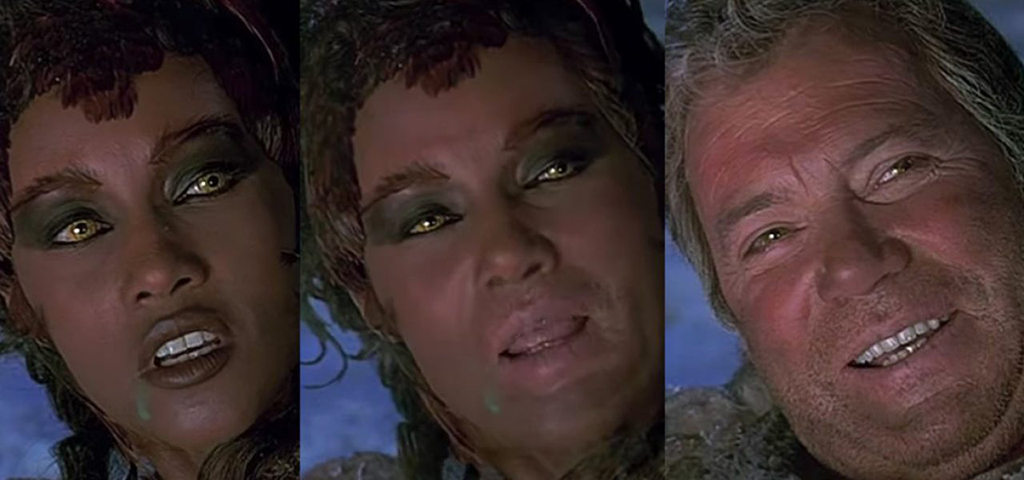
\includegraphics[width=\textwidth]{ch-sistemasABC/images/ch-morphing/old/artist_morphing_01.png}
        \caption{1991. Fotogramas de \textit{Star Trek VI}.}
    \end{subfigure}
    \newline
    \begin{subfigure}[b]{0.8\textwidth}
        \centering
        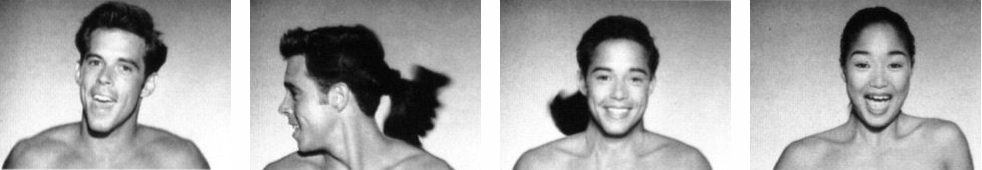
\includegraphics[width=\textwidth]{ch-sistemasABC/images/ch-morphing/old/artist_morphing_02.png}
        \caption{1991. \textit{Black and white} - vídeo musical Michael Jackson.}
    \end{subfigure}
    \caption{Ejemplos de uso del \textit{morphing} en la industria audiovisual.}
    \label{fig:first_morphing_samples}
\end{figure}

Debido a los buenos resultados conseguidos fusionando caras y a la dificultad que supone visualmente detectar si una imagen ha sido manipulada \cite{beale1995categorical} \cite{levin2000categorical} \cite{robertson2018detecting}, en poco tiempo, el \gls{morphing} paso de ser un recurso artístico a convertirse en una herramienta ideal para cometer delitos. La falsificación de documentos mediante \gls{morphing} se ha convertido en un gran problema \cite{scherhag2017vulnerability} \cite{makrushin2017automatic} y especialmente en documentos sensibles, como los pasaportes \cite{ferrara2014magic}.

En este capitulo se propone un mecanismo de \GLS{MAD} diferencial con \gls{de-morphing} que requiere de dos imágenes. En el caso de los sistemas \GLS{ABC}: La imagen almacenada en el \gls{eMRTD} (\gls{chip}), posiblemente alterada, y la imagen capturada en el cruce (\gls{vivo}) del viajero que se dispone a cruzar la frontera.

Cuando la imagen \gls{chip} de un pasaporte ha sido alterada, la imagen resultante del \gls{de-morphing} entre  la \gls{chip} y la \gls{vivo} del viajero \gls{impostor} tiene los rasgos del viajero \gls{genuino}, lo que permite detectar cuando un pasaporte ha sido atacado con \gls{morphing}.

La solución propuesta se implementa mediante una arquitectura de \textit{Convolutional Neural Network} (\GLS{CNN}) basada en dos codificadores y un decodificador (\GLS{DMN}). La tasa de obtenida es alta, en comparación con los valores alcanzados por otras propuestas en la literatura, incluso con imágenes de poca calidad. Algo crucial en sistemas \GLS{ABC} ya que las imágenes almacenadas en los \gls{eMRTD} han sido previamente impresas y escaneadas.

El trabajo se organiza de la siguiente manera: El problema de los ataques de \gls{morphing} en los sistemas \GLS{ABC} se presenta en la Sección \ref{sec:VerificationMorphingAttack}. A continuación en la sección \ref{sec:de-morphingApproach} se describe la solución propuesta. Y finalmente en las Secciones \ref{sec:morphingResultados} y \ref{sec:MorphingConclusiones}  presentan los resultados obtenidos y las conclusiones.

 %%% SISTEMAS DE VERICACION FACIAL CON ATAQUES DE MORPHING
\section{Sistemas de verificación facial frente a ataques de \textit{morphing}} \label{sec:VerificationMorphingAttack}

\begin{figure}[t!]
    \centering
    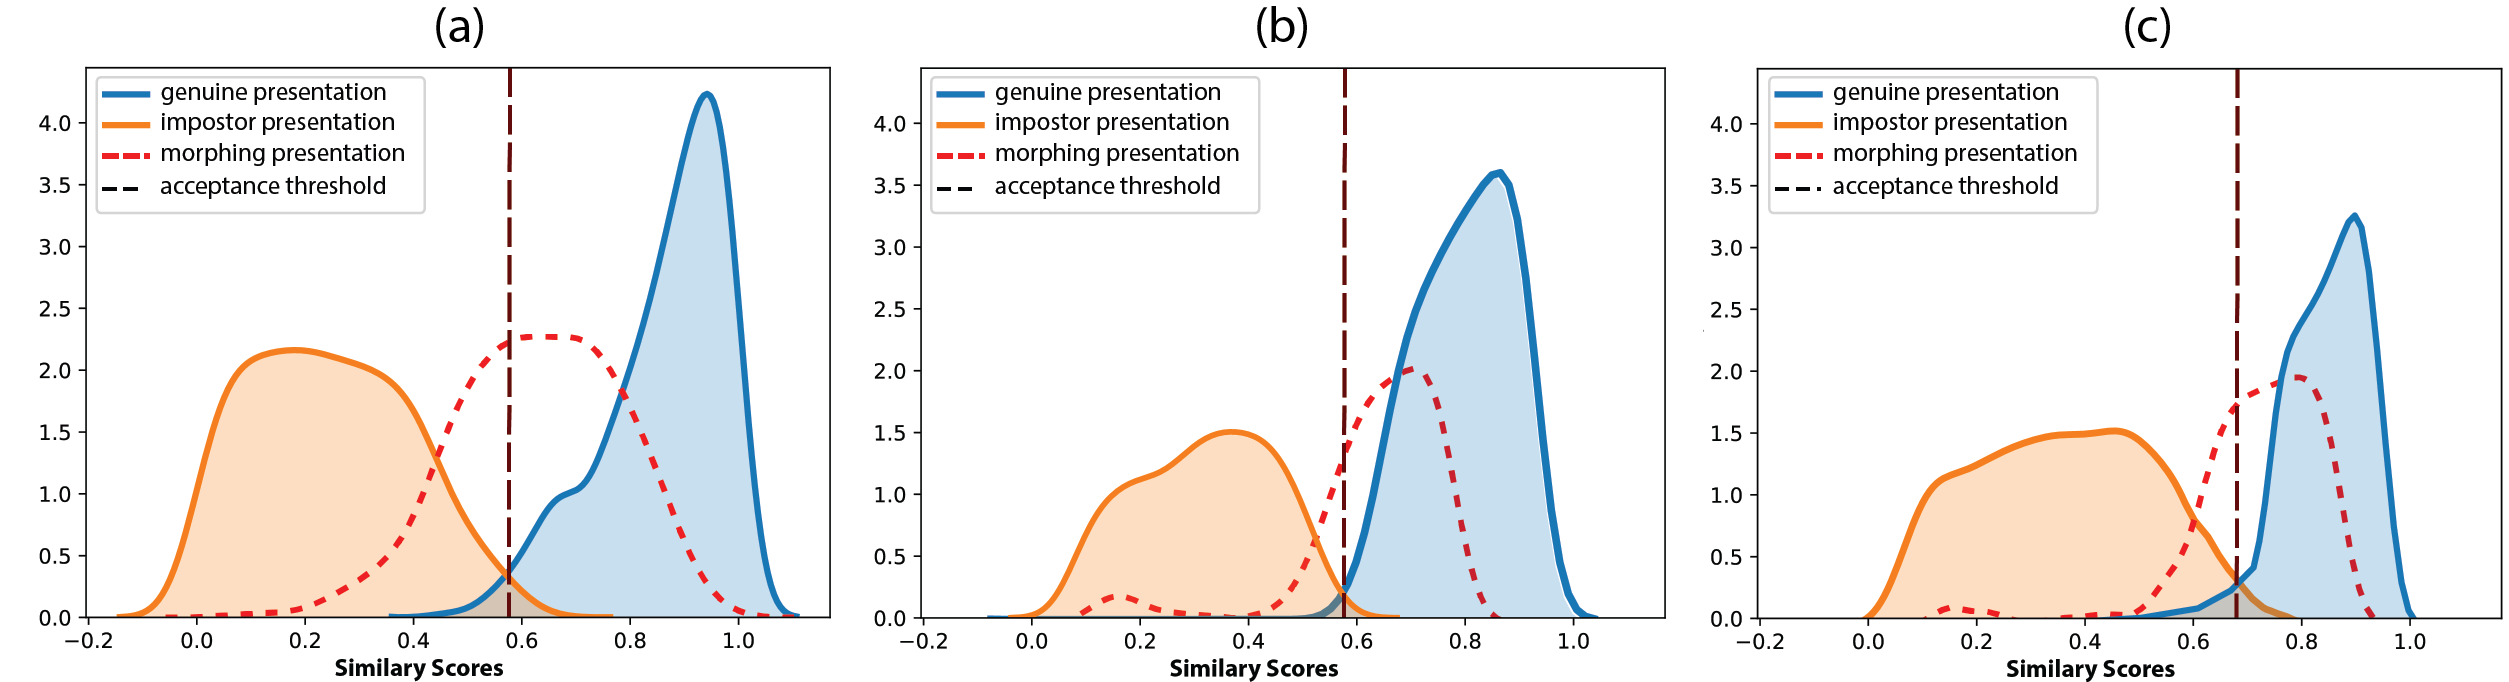
\includegraphics[width=1\textwidth]{ch-sistemasABC/images/ch-morphing/COMPARATIVA_DE_LOS_SCORES_DE_FACE_NET.png}
    \caption{Distribución de los \textit{scores} de similitud de \Gls{FaceNet} \cite{schroff2015facenet} calculados con imágenes de: (a) \Gls{FRAV-Morphing-Test} (b) \Gls{FRAV-Morphing-Test-PS-300} y (c) \Gls{FRAV-Morphing-Test-PS-150}.}
    \label{fig:FaceNetProbabilities}
\end{figure}

\begin{figure}[t!]
    \centering
    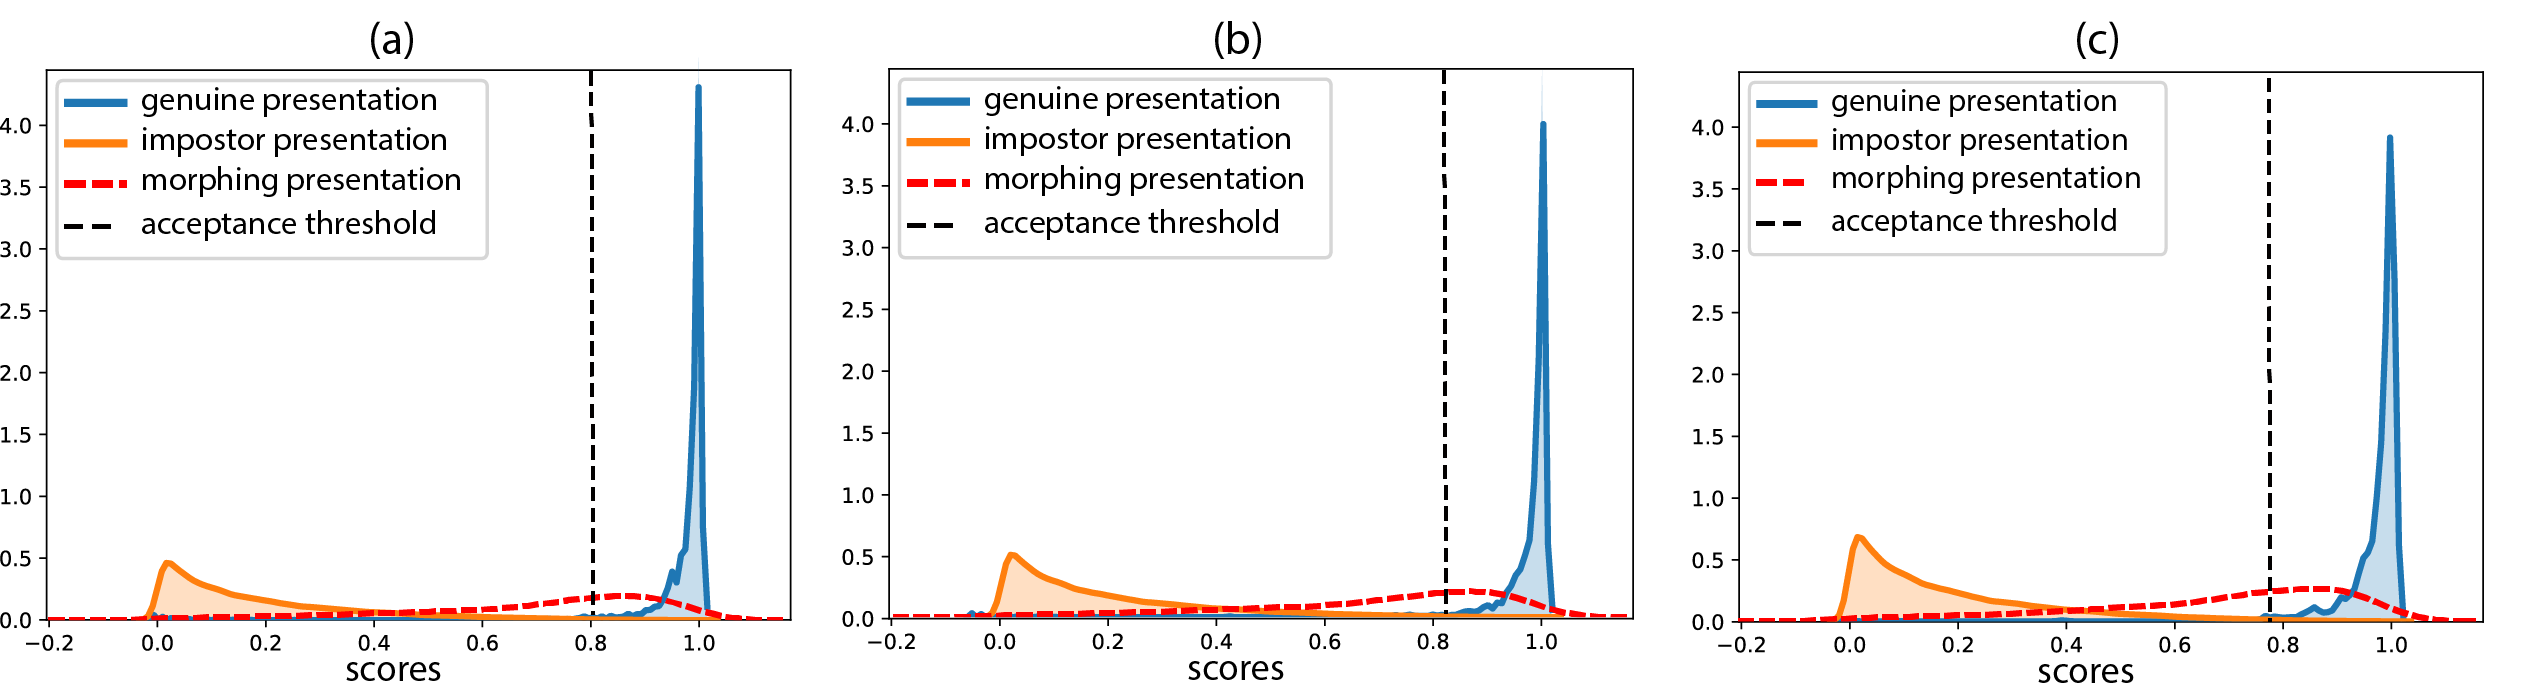
\includegraphics[width=1\textwidth]{ch-sistemasABC/images/ch-morphing/COMPARATIVA_DE_LOS_SCORES_DE_LUXAND.png}
    \caption{Distribución de los \textit{scores} de verificación con un \GLSpl{COT} calculados con imágenes de: (a) \Gls{FRAV-Morphing-Test} (b) \Gls{FRAV-Morphing-Test-PS-300} y (c) \Gls{FRAV-Morphing-Test-PS-150}.}
    \label{fig:LuxandProbabilities}
\end{figure}

La mayor parte de los sistemas de verificación facial no están preparados para hacer frente a los ataques de \gls{morphing} \cite{gomez2017your} \cite{spreeuwers2018towards} como puede verse en las figuras \ref{fig:FaceNetProbabilities} y \ref{fig:LuxandProbabilities}. En la Fig. \ref{fig:FaceNetProbabilities} se muestran las distribuciones de los \textit{scores} obtenidos con \gls{FaceNet} \cite{SandbergFaceNet}, un sistema de reconocimiento facial de código abierto y en Fig. \ref{fig:LuxandProbabilities} las obtenidas con un \GLSpl{COT} de referencia en la literatura \cite{ferrara2014magic}. En cada una de las figuras se presentan tres gráficas: a la izquierda los resultados obtenidos con las imágenes de la base de datos \Gls{FRAV-Morphing-Test}, en el centro los resultados con \Gls{FRAV-Morphing-Test-PS-300} y a la derecha con \Gls{FRAV-Morphing-Test-PS-150}. Cada gráfica, a su vez, presenta tres curvas: la distribución de \textit{scores} obtenidos con viajeros genuinos (azul, un viajero con su documentación), la segunda los obtenidos con viajeros impostores (naranja, un impostor con la documentación de otro viajero), y la tercera, los obtenidos con ataques de \gls{morphing} (lineas rojas discontinuas, un impostor con la documentación de otro viajero pero manipulada con \gls{morphing}).

En todas las gráficas se observa que los \textit{scores} de los individuos genuinos y de los impostores están bien separadas, y es posible definir un umbral de aceptación adecuado (lineas negras discontinuas) para lograr altas tasas de precisión tanto con \gls{FaceNet} como con el \GLSpl{COT}. Los \textit{scores} inferiores al umbral, son presentaciones genuinas mientras que los \textit{scores} que están por encima del umbral son de impostores. Pero el problema está en fijar el umbral de aceptación que permita distinguir si se produce o no un ataque de \gls{morphing} ya que los \textit{scores} de \gls{morphing} se superponen a los \textit{scores} de genuinos e impostores.

El problema con la superposición de los \textit{scores} es aun más complejo cuando las imágenes han sido impresas y escaneadas (como \Gls{FRAV-Morphing-Test-PS-300} y \Gls{FRAV-Morphing-Test-PS-150}. Por lo tanto, esta claro que es obligatorio el uso de sistemas \GLS{MAD} para prevenir ataques.


\subsection{Sistemas MAD con imágenes impresas y escaneadas} \label{ref:MADsystemUnderPrintScan} %%% DEMORPHINF CON IMAGENES IMPRESAS ESCANEDAS

\begin{figure}[t!]
    \centering
    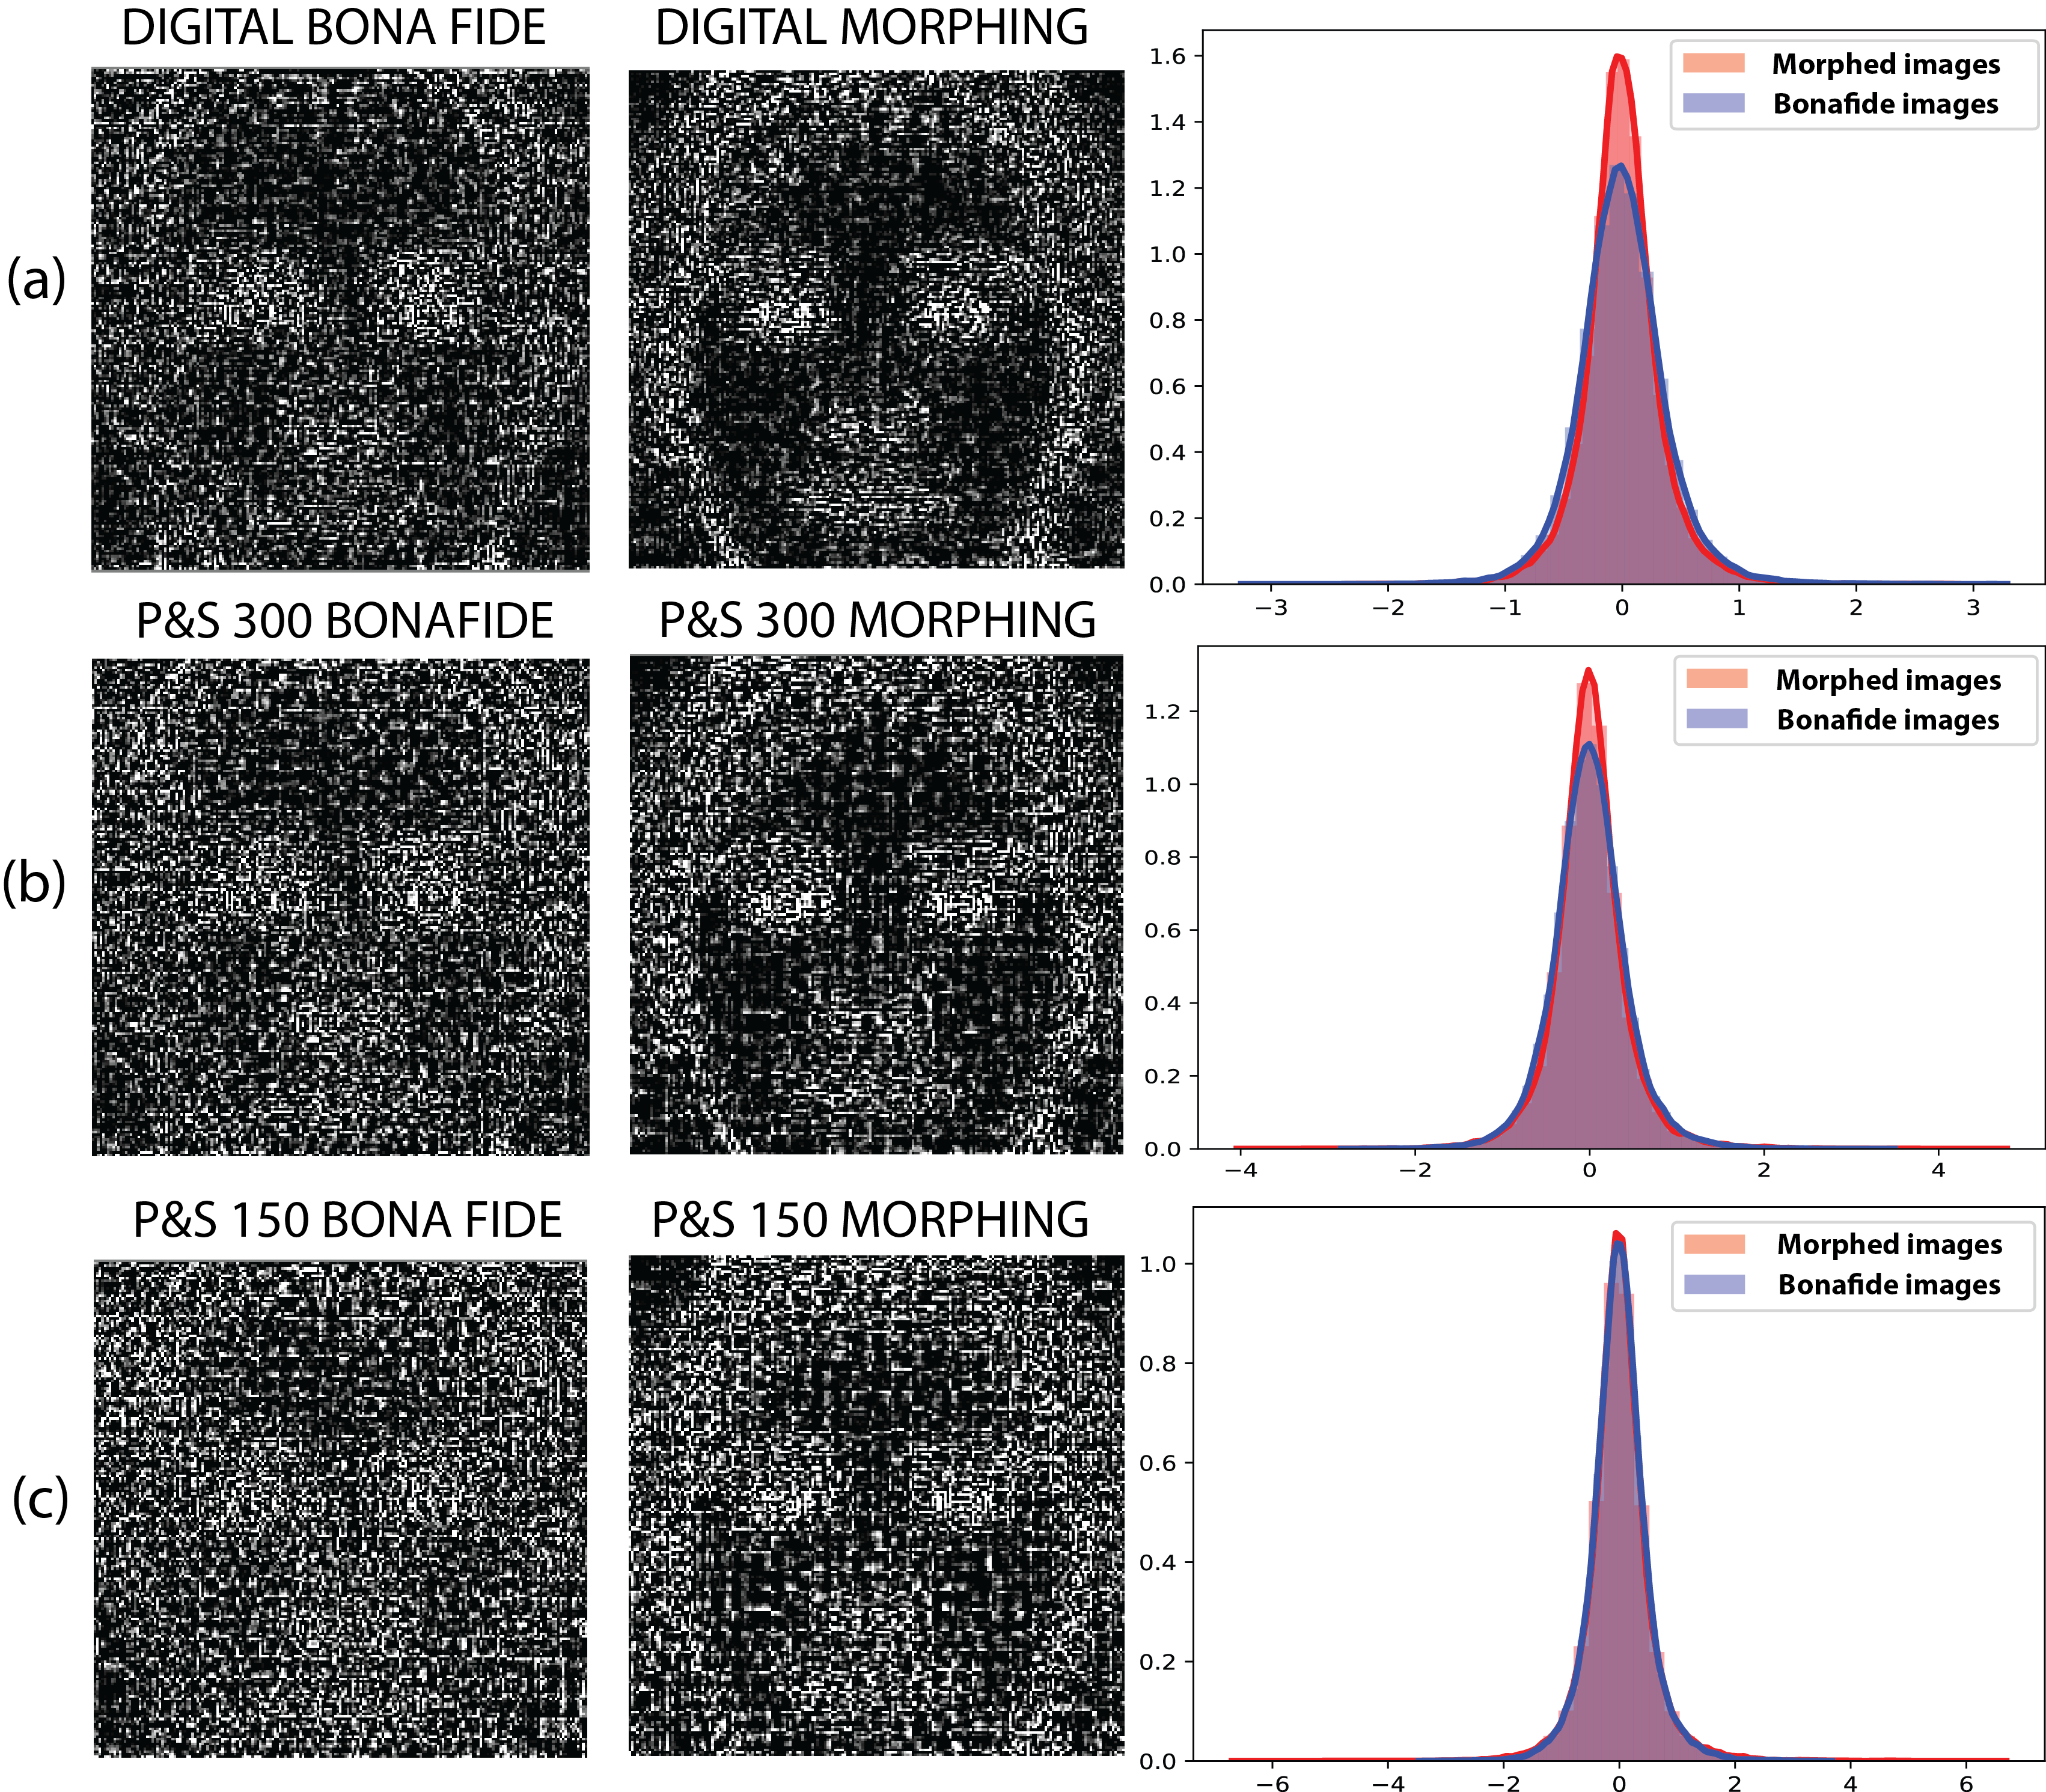
\includegraphics[width=0.7\textwidth]{ch-sistemasABC/images/ch-morphing/COMPARATIVA_PRNU_CON_BONAFIDE_MORPHING.png}
    \caption{Imagen \GLS{PRNU} \cite{lukas2006digital} de imágenes con \gls{morphing} y de imágenes \gls{bona-fide}. Y comparación de los histogramas \GLS{PRNU} medios de $100$ imágenes con \gls{morphing} y  $100$ imágenes \gls{bona-fide} de las base de datos: (a) \Gls{FRAV-Morphing-Test}, (b) \Gls{FRAV-Morphing-Test-PS-300} y (c) \Gls{FRAV-Morphing-Test-PS-150}.}
    \label{fig:PRNU_COMPARATIVE}
\end{figure}

Gran parte de los métodos usados para la detección de ataques de presentación de tipo \gls{morphing} se basan en características de las imágenes muy sensibles al ruido (\GLS{LBP} \cite{jassim2018automatic}, \cite{spreeuwers2018towards}, \cite{damer2018morgan}, \cite{wandzik2018morphing}; \GLS{PRNU} \cite{debiasi2018prnu}, \cite{debiasi2018prnuvar}, \GLS{SIFT} \cite{lowe2004distinctive}, \cite{neubert2017face}), por lo que no resultan efectivos con imágenes con poca calidad, como imágenes impresas y escaneadas \cite{ferrara2019face}, \cite{raghavendra2017face}, Uno de estos métodos es por ejemplo el propuesto por \textit{Debiasi, Luca et al}. \cite{debiasi2018prnuvar}, \cite{debiasi2018prnu}, que propone como características discriminantes, histogramas \textit{Photo Response Non-Uniformity} (\GLS{PRNU}) \cite{lukas2006digital}, lo que se conoce como la huella dactilar de la imágenes.

Para poner a prueba este método y a su vez evaluar la resistencia a la detección que tienen las imágenes de las bases de datos usadas para futuros experimentos, en la Fig \ref{fig:PRNU_COMPARATIVE}) se presenta un análisis realizado del \GLS{PRNU} de imágenes \gls{chip} de (a) \Gls{FRAV-Morphing-Test}, (b) \Gls{FRAV-Morphing-Test-PS-300}, y (c) \Gls{FRAV-Morphing-Test-PS-150}. A la izquierda se presentan un par de muestras con los patrones \GLS{PRNU} de imágenes \gls{chip} \gls{bona-fide} y de imágenes \gls{chip} con \gls{morphing}. Y a la derecha de cada par de muestras, un gráfico con el histograma \gls{PRNU} medio de cien imágenes \textit{<<\gls{chip}>>} \gls{bona-fide} (rojo) enfrentado al de cien imágenes \textit{<<\gls{chip}>>} con \gls{morphing} (azul). Con la base de datos \Gls{FRAV-Morphing-Test} existe una pequeña diferencia entre los los histogramas \GLS{PRNU}, lo que indica que sería posible distinguir entre \gls{bona-fide} y \gls{morphing}. En \Gls{FRAV-Morphing-Test-PS-300} esta diferencia se reduce, y ya en la base de datos \Gls{FRAV-Morphing-Test-PS-300} los histogramas son idénticos lo que impide completamente la detección de ataques con este método.

%%% DEMORPHIG DMN
\section{Enfoque \textit{de-morphing}} \label{sec:de-morphingApproach}

El objetivo de un proceso \gls{de-morphing} es separar las dos identidades que se han fusionado en un \gls{morphing}. Para entender como puede usarse el proceso \gls{de-morphing} como mecanismo de \GLS{MAD} para detectar si una imagen ha sido manipulada se deben tener en cuanta dos propiedades del \gls{de-morphing}: 

 \renewcommand{\labelenumi}{\alph{enumi}}
 \renewcommand{\labelenumi}{\theenumi)}
\begin{enumerate}
\item 
Idealmente, como muestra la ecuación \ref{eq:demorph_ideal} (donde C es el morphing de las identidades de A y B), con una imagen \gls{morphing} y la imagen de una de las dos identidades fusionadas, se consigue extraer la imagen de la otra identidad. Pero normalmente no se dispone de la imagen original con la que se realizó el \gls{morphing} con lo que al aplicar el \gls{de-morphing}, con una imagen aproximada de la identidad, no se obtiene una imagen nítida de la otra identidad, pero si una aproximación, como se ve en la ecuación \ref{eq:demorph_no_ideal}.

\begin{equation}\label{eq:demorph_ideal}
  A \cap B = C; C - A = B;C - B = A
\end{equation}

\begin{equation}\label{eq:demorph_no_ideal}
  A \cap B = C; C - \tilde{A} \approx B;C - \tilde{B} \approx A
\end{equation}

\item
Idealmente, el resultado de aplicar el \gls{de-morphing} a una imagen sombre si misma,  es la misma imagen (ecuación \ref{eq:demorph_reflexivo_ideal}). Pero si la imagen con la que se aplica el \gls{de-morphing} no idéntica el resultado será una aproximación de la misma imagen, como se ve en la ecuación \ref{eq:demorph_reflexivo_no_ideal}. 

\begin{equation}\label{eq:demorph_reflexivo_ideal}
  A - A = A;B - B = B
\end{equation}

\begin{equation}\label{eq:demorph_reflexivo_no_ideal}
  A - \tilde{A} \approx A;B - \tilde{B} \approx B
\end{equation}

\end{enumerate}

El proceso de \gls{de-morphing} puede usarse para detectar si una imagen es un \gls{morphing}. Al aplicar el \gls{de-morphing} al posible \gls{morphing} con una imagen de la misma identidad, si la imagen resultante conserva la identidad, no hay \gls{morphing}, mientras que si no la conserva, se puede afirmar que la existe un \gls{morphing} con identidad resultante. Verificado el resultado del \gls{de-morphing} se puede detectar si una imagen es un \gls{morphing}. 

\begin{equation}\label{eq:similarOrNot}
\begin{split}
\textit{Si   } &C - A \sim A \Rightarrow \textit{  C no es un \gls{morphing}}\\
\textit{Si   } &C - A \nsim A \Rightarrow \textit{  C es un \gls{morphing}}
\end{split}
\end{equation}

\begin{figure}[t!]
    \centering
    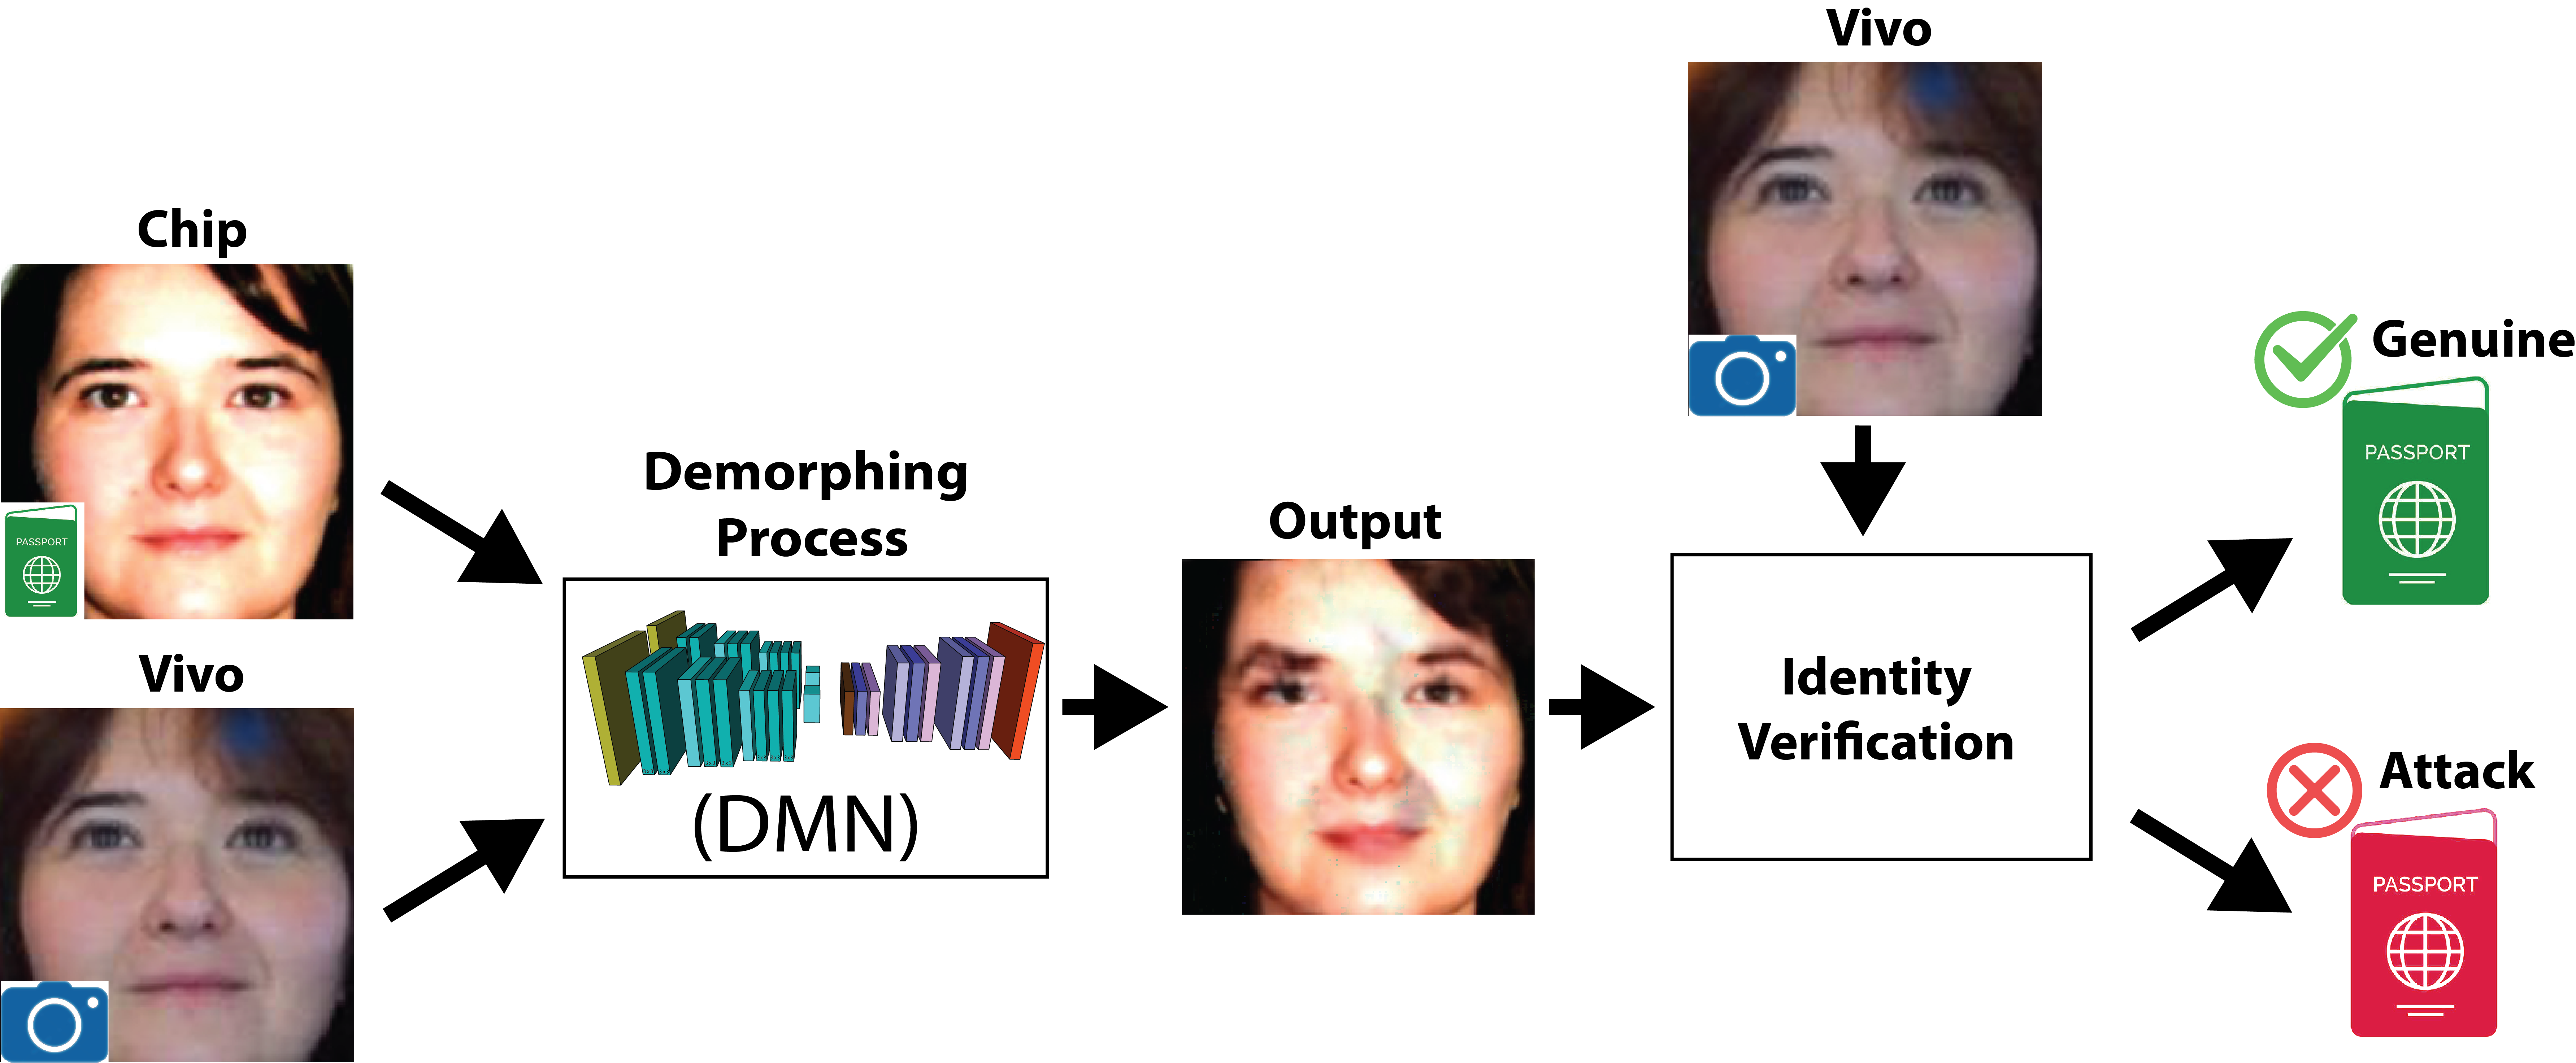
\includegraphics[width=1\textwidth]{ch-sistemasABC/images/ch-morphing/ProcesoGeneralDemorphingVerificacion.png}
    \caption{Proceso \gls{de-morphing} y procesos de verificación de la identidad resultante.}
    \label{fig:de-morphingConYSinMorphing}
\end{figure}

En el escenario real de un sistema \GLS{ABC} (ver Fig. \ref{fig:de-morphingConYSinMorphing}), si el resultado del proceso \gls{de-morphing} entre la imagen \gls{chip} y la imagen \gls{vivo} verifica los rasgos biométricos de la imagen \gls{vivo} en viajero es el propietario \gls{genuino} del documento, mientras que si el resultado del \gls{de-morphing} no verifica, el viajero es un \gls{impostor} y el documento ha sido alterado con la imagen de un \gls{morphing} entre el propietario \gls{genuino} y el viajero \gls{impostor}.

%%% PROCESO DEMORPHING
\section{Proceso de \textit{de-morphing}} \label{ref:de-morphingProcess}

\begin{figure}[t!]
    \centering
    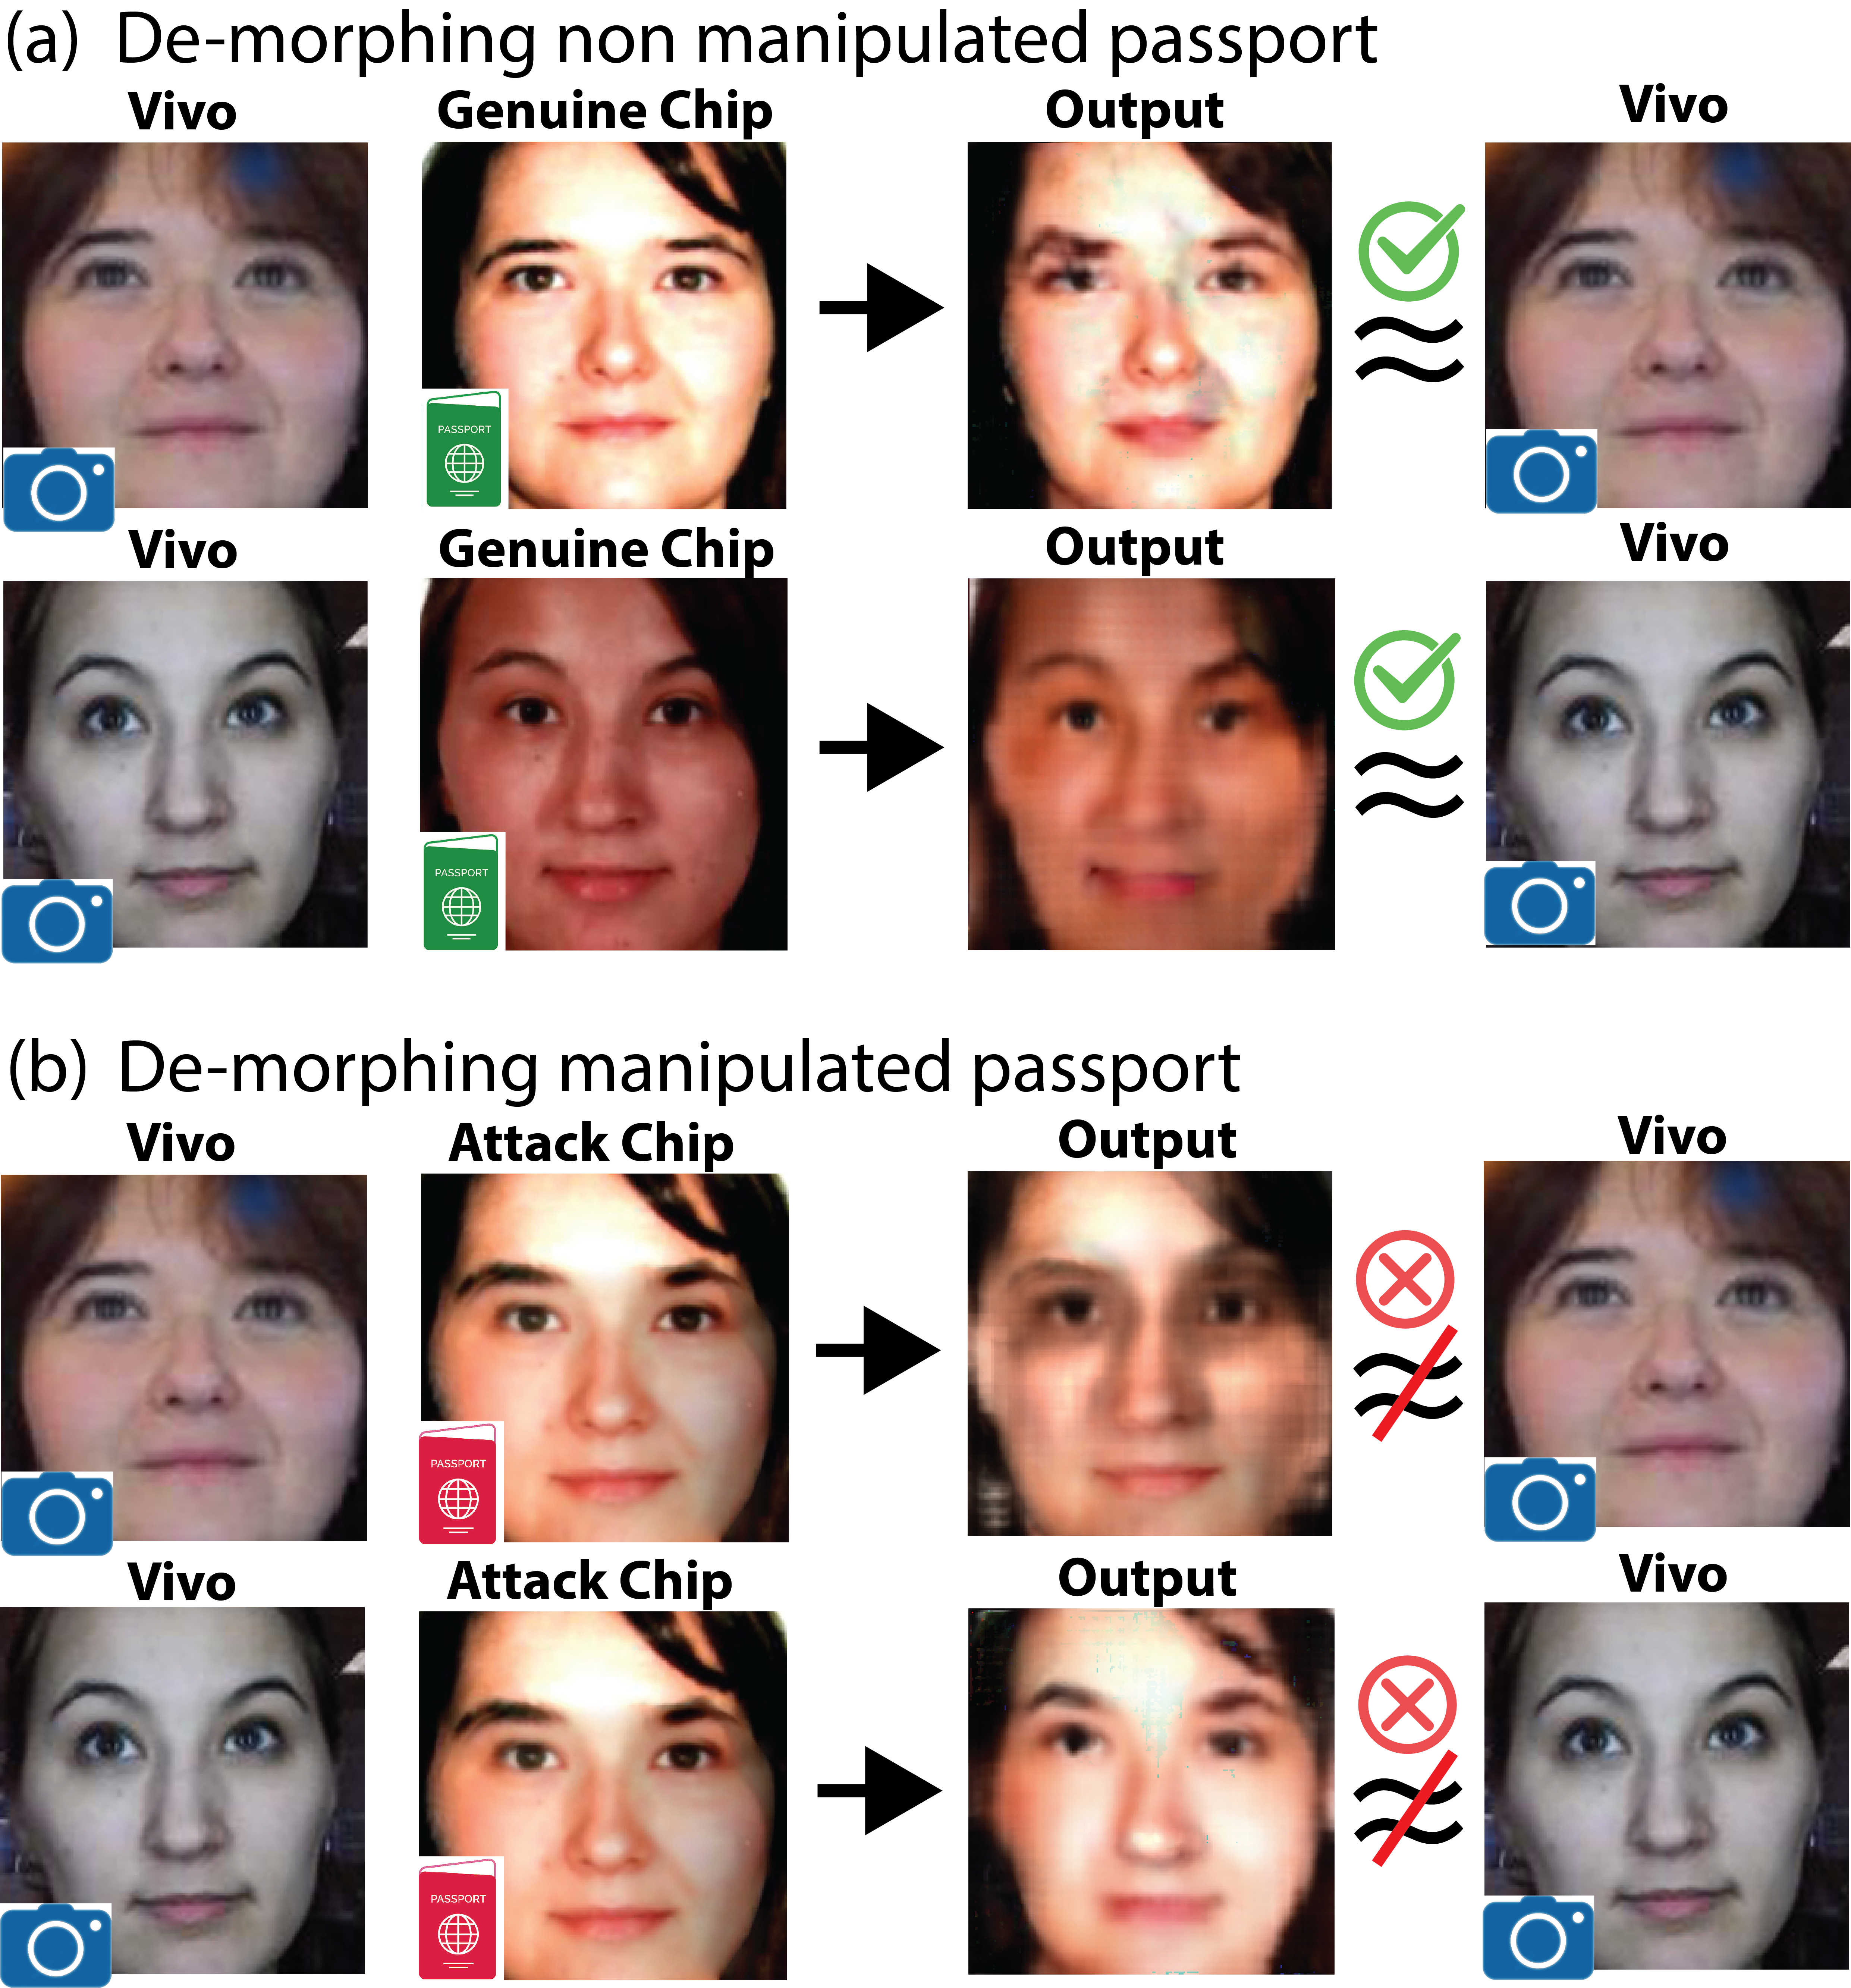
\includegraphics[width=0.8\textwidth]{ch-sistemasABC/images/ch-morphing/DemorphingCrisBeaSimple.png}
    \caption{Proceso de \gls{de-morphing} en pasaportes (a) sin ataque \gls{morphing} y (b) con \gls{morphing}.}
    \label{fig:SamplesImagesde-morphing}
\end{figure}

\begin{figure}[t!]
    \centering
    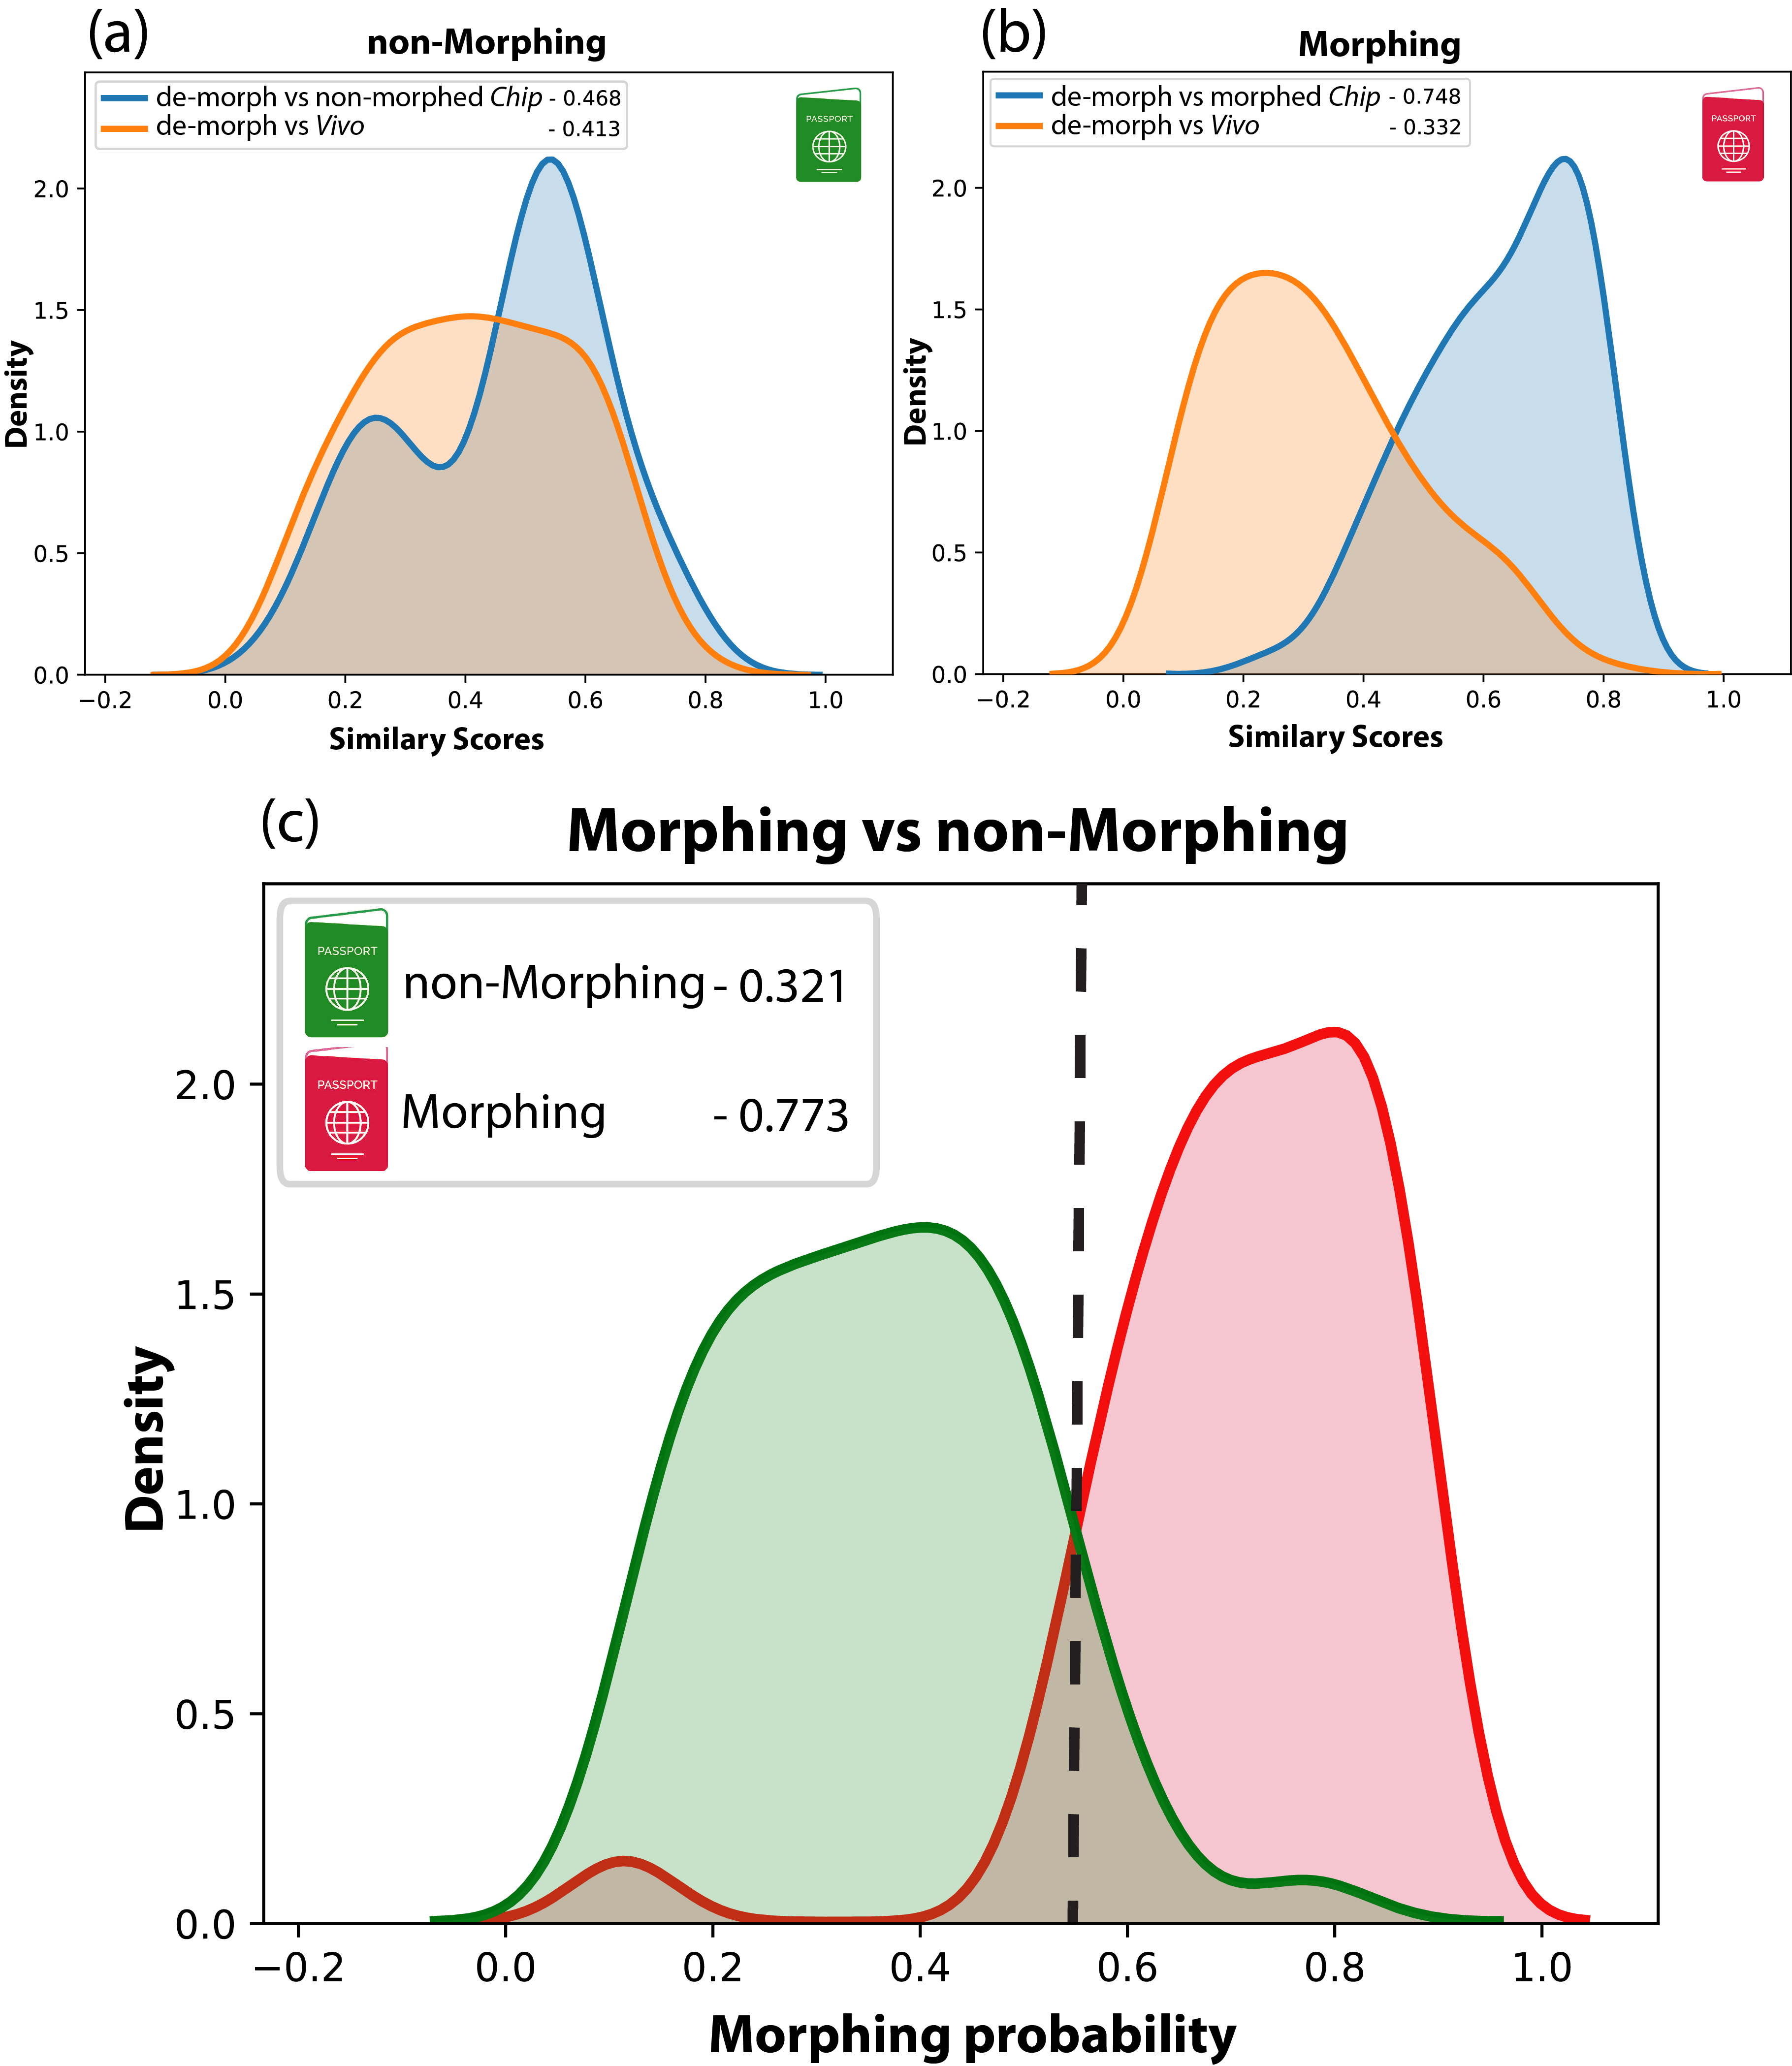
\includegraphics[width=0.8\textwidth]{ch-sistemasABC/images/ch-morphing/DIS_COMPARA_DEMO_CHIP_DEMO_VIVO_AND_MORPHING_TO_BONAFIDE.png}
    \caption{Distribución de los \textit{scores} de similitud de \gls{FaceNet} \cite{schroff2015facenet} entre la imagen \gls{de-morphing} y la imagen \gls{vivo} (a) cuando la imagen \gls{chip} no tiene \gls{morphing} y (b) cuando la imagen \gls{chip} tiene \gls{morphing}. (c) Distribución probabilidad cuando hay \gls{morphing} y cuando no hay \gls{morphing}}
    \label{fig:Distancesde-morphing}
\end{figure}

Fig. \ref{fig:SamplesImagesde-morphing} describe el comportamiento del proceso con pasaportes manipulados (a) y no manipulados (b). Se utilizan pictogramas: El pasaporte verde significa una imagen genuina, el pasaporte rojo una imagen fraudulenta con \gls{morphing} y el símbolo de la cámara azul para señalar la imagen \gls{vivo} capturada en el\GLS{ABC}.


\color{cyan}
% En la ecuación \ref{eq:similarOrNot}, se ilustran los procesos de \textit{\gls{morphing}} y \textit{\gls{de-morphing}}. Las operaciones en los \textit{sets} ayudan a entender el papel que las diferentes imágenes (\textit{<<\gls{vivo}>>} o de \textit{<<chip>>}) juegan en el proceso. 

% \begin{equation}\label{eq:similarOrNot}
%   A \cap B = C; C - A \sim B; C - A \nsim A
% \end{equation}

% La intersección de dos imágenes (A y B) es la representación del proceso de \textit{\gls{morphing}}, donde C es la imagen \textit{\gls{morphing}}. La diferencia entre C-A representa el proceso de \textit{\gls{de-morphing}}. C-A debe ser una imagen similar a B (en el caso de que C sea una imagen transformada); sin embargo C-A no será similar a la imagen A. Si se presenta una imagen transformada en una puerta \GLS{ABC}, sólo se obtiene la imagen C y A (C del \textit{chip} y A de la imagen \textit{\gls{vivo}}). Si C-A no es similar a A, se puede suponer que se ha utilizado una imagen B para componer un ataque de \textit{\gls{morphing}}. 

% Por lo tanto, si la instantánea de salida comparada y la imagen del \textit{\gls{vivo}} son similares y la imagen del \textit{\gls{vivo}} es también similar a la imagen del \textit{chip} antes del proceso de \textit{\gls{de-morphing}}, entonces se puede notar que la salida no es un ataque de \textit{\gls{morphing}}, como se ilustra en la Fig. \ref{fig:SamplesImagesde-morphing} (a)
% % % Editor de control de calidad: Por favor, asegúrese de que el significado deseado se ha mantenido en las ediciones de la frase anterior.
% Sin embargo, si la imagen de salida no es similar a la imagen \textit{\gls{vivo}}  (independientemente de la similitud con la imagen \textit{chip} antes del proceso de \textit{\gls{de-morphing}}), entonces se realizó un ataque de \textit{\gls{morphing}}, como se muestra en la Fig.\ref{fig:SamplesImagesde-morphing} (b).
\color{black}

La salida del proceso de \gls{de-morphing} se verifica con las imágenes \gls{vivo} y \gls{chip}. En la Fig. \ref{fig:Distancesde-morphing}, se muestran las distribuciones de los \textit{scores} obtenidos en dichas verificaciones: Cuando el \gls{de-morphing} se aplica en un \gls{chip} no manipulado (a) y cuando el \textit{<<\gls{chip}>>} es un \gls{morphing} (b),  

Cuando un \textit{<<chip>>} no ha sido alterado (Fig. \ref{fig:Distancesde-morphing} (a)), el \textit{score} de verificación entre el resultado del \gls{de-morphing} y el \gls{vivo} es equivalente al \textit{score} de variación entre el \gls{de-morphing} y el \textit{<<\gls{chip}>>}. En otras palabras al aplicar \gls{de-morphing} a un pasaporte no manipulado, el aspecto de la imagen resultante continua pareciéndose al \gls{chip} y al \gls{vivo}.

Sin embargo, cuando el \gls{chip} es un \gls{morphing} (Fig. \ref{fig:Distancesde-morphing} (b)), el \textit{score} de verificación entre el resultado del \gls{de-morphing} y el \gls{vivo} es menor que el \textit{score} de verificación entre el resultado del \gls{de-morphing} y el \gls{chip}. En otras palabras al aplicar un \gls{de-morphing} a un pasaporte manipulado, el aspecto de la imagen resultante aunque se siga pareciendo a la imagen del pasaporte ya no se parece al \gls{vivo}.

Teniendo en cuenta los \textit{scores} de verificación obtenidos después de aplicar el \gls{de-morphing} se puede establecer un \textit{score} de detección que determine la probabilidad de que el pasaporte haya sido manipulado o no. En Fig. \ref{fig:Distancesde-morphing} (c)) se presenta la distribución de estos \textit{scores} de detección en pasaportes con \gls{morphing} y sin \gls{morphing}. 

\begin{figure}[t!]
    \centering
    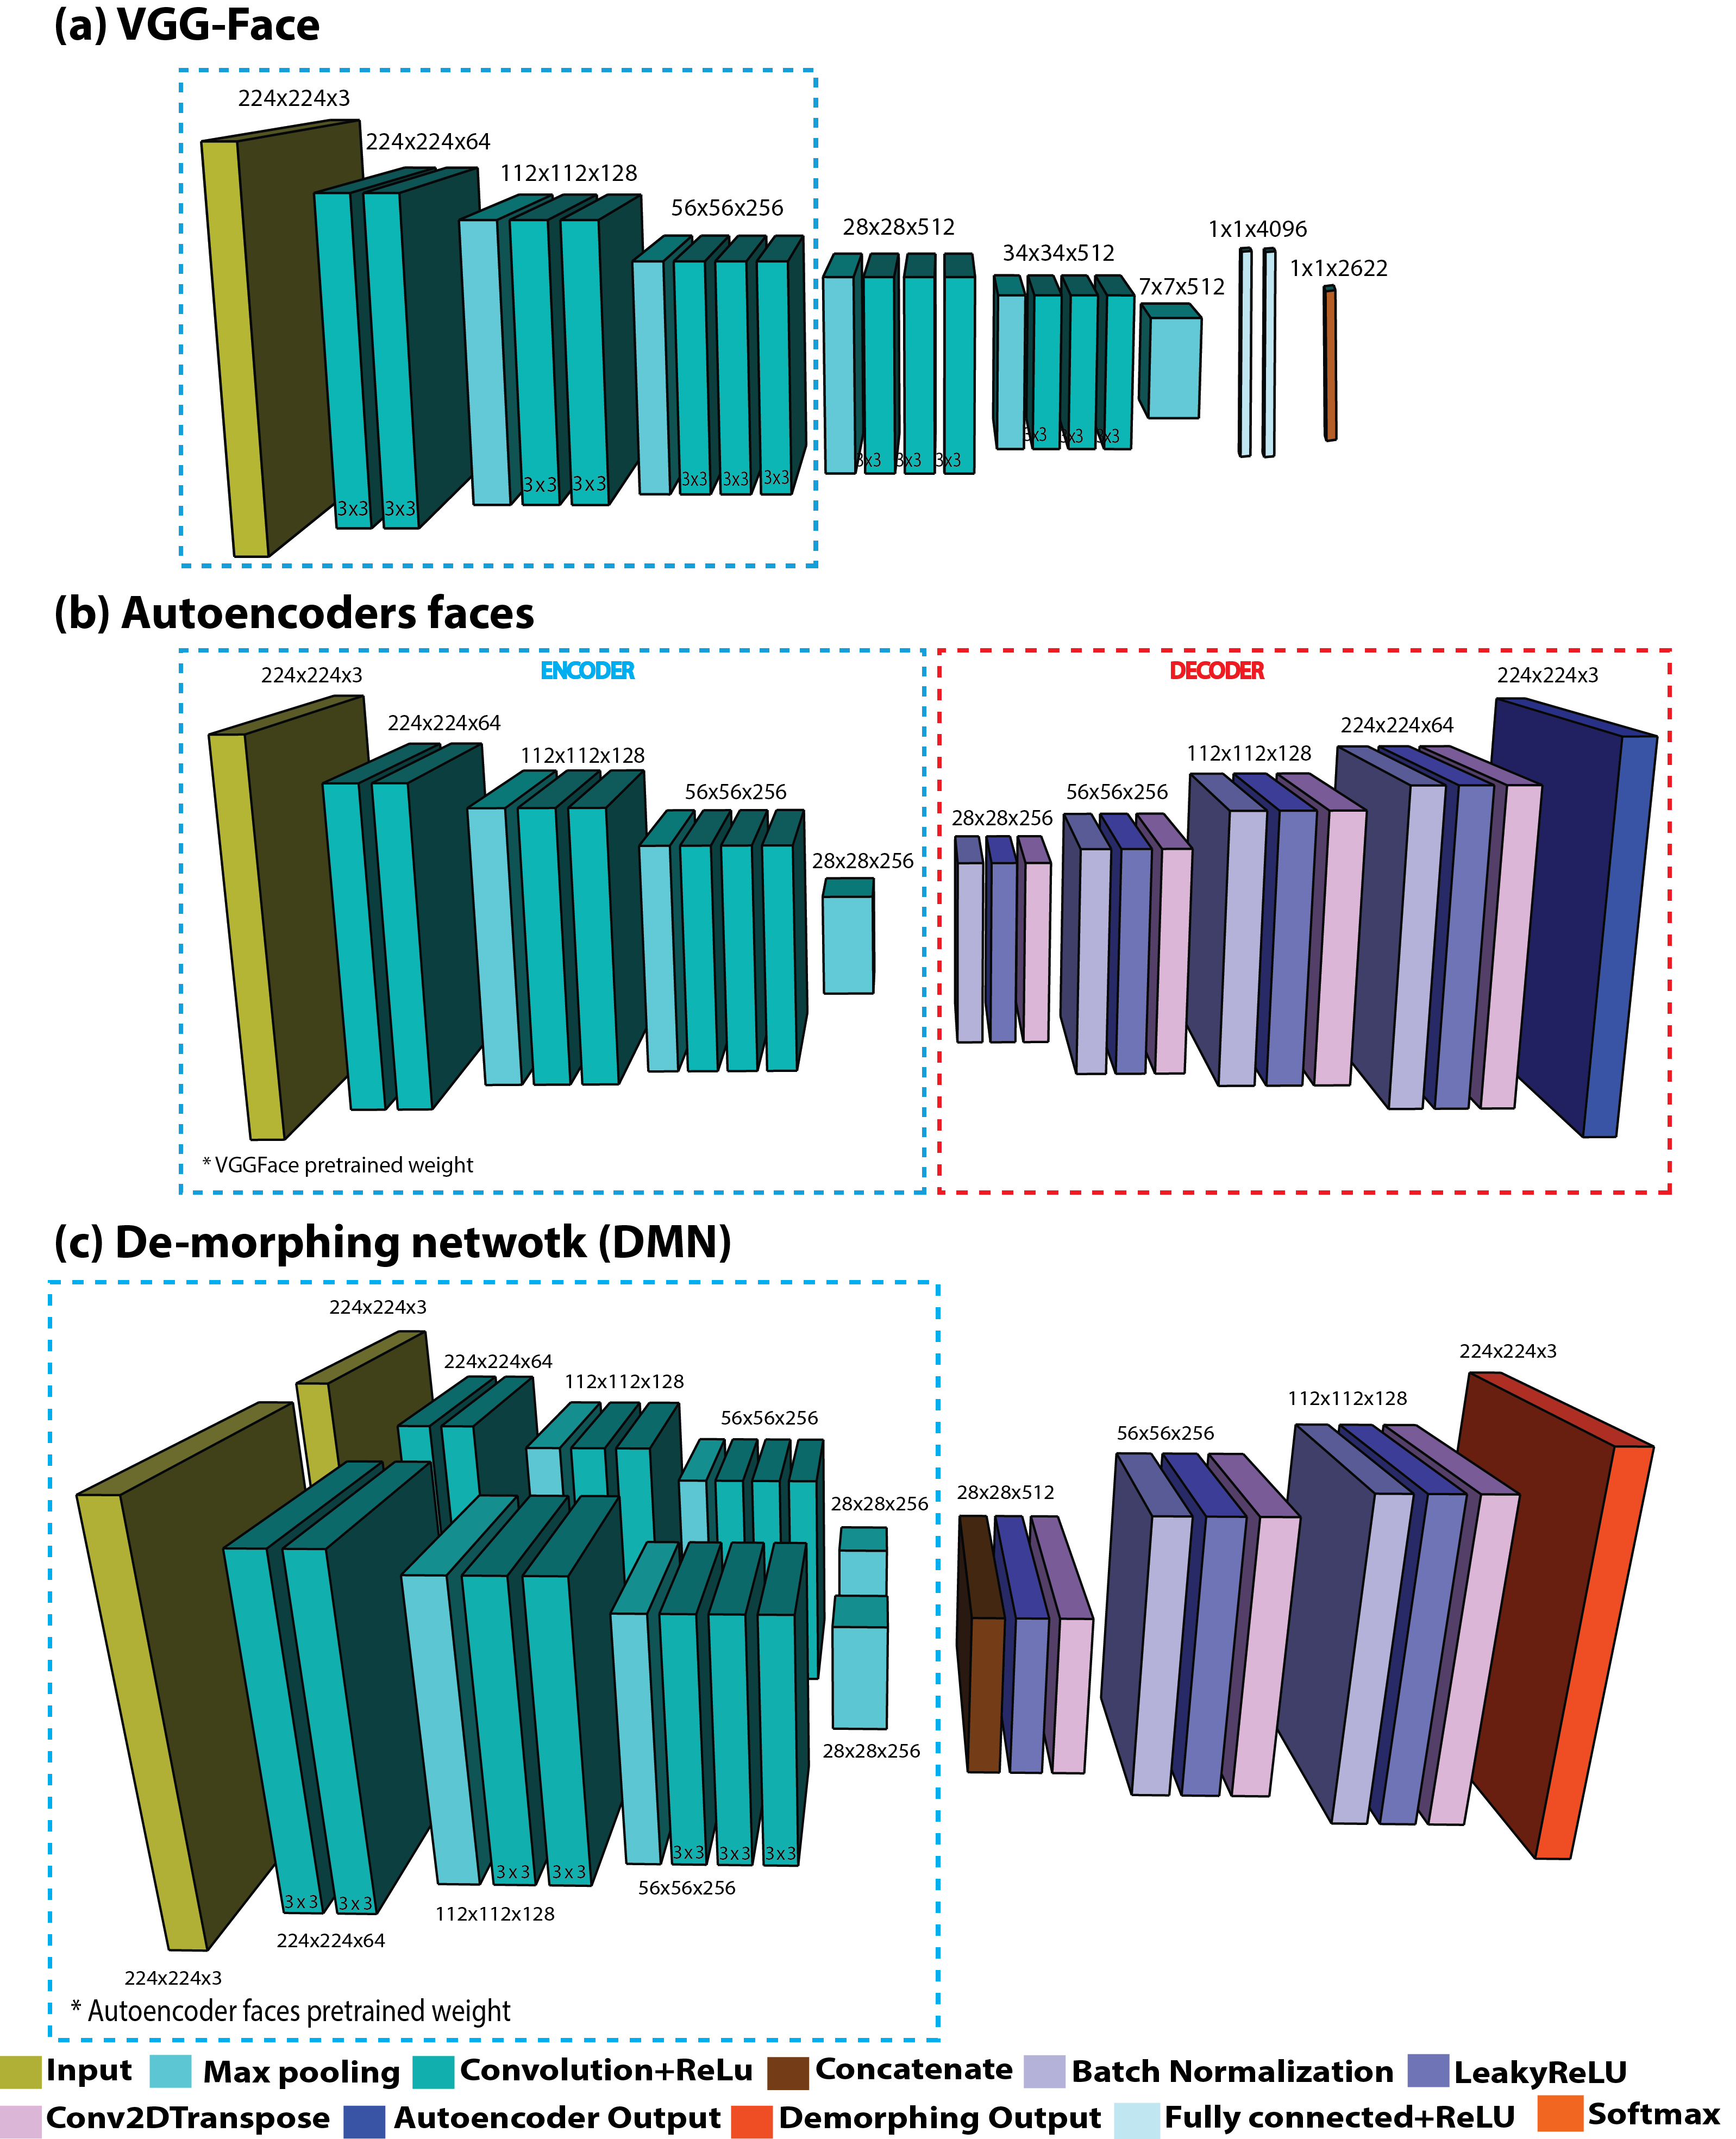
\includegraphics[width=1\textwidth]{ch-sistemasABC/images/ch-morphing/ARQUITECTURAS_LEYENDA_GRANDE.png}
    \caption{Arquitecturas \GLS{CNN}: (a) \GLS{VGG-Face} \cite{parkhi2015deep}, (b) \Gls{autoencoder} y (c) \textit{\Gls{de-morphing} network} (\GLS{DMN}).}
    \label{fig:Arquitecturas}
\end{figure}

\begin{figure}[t!]
    \centering
    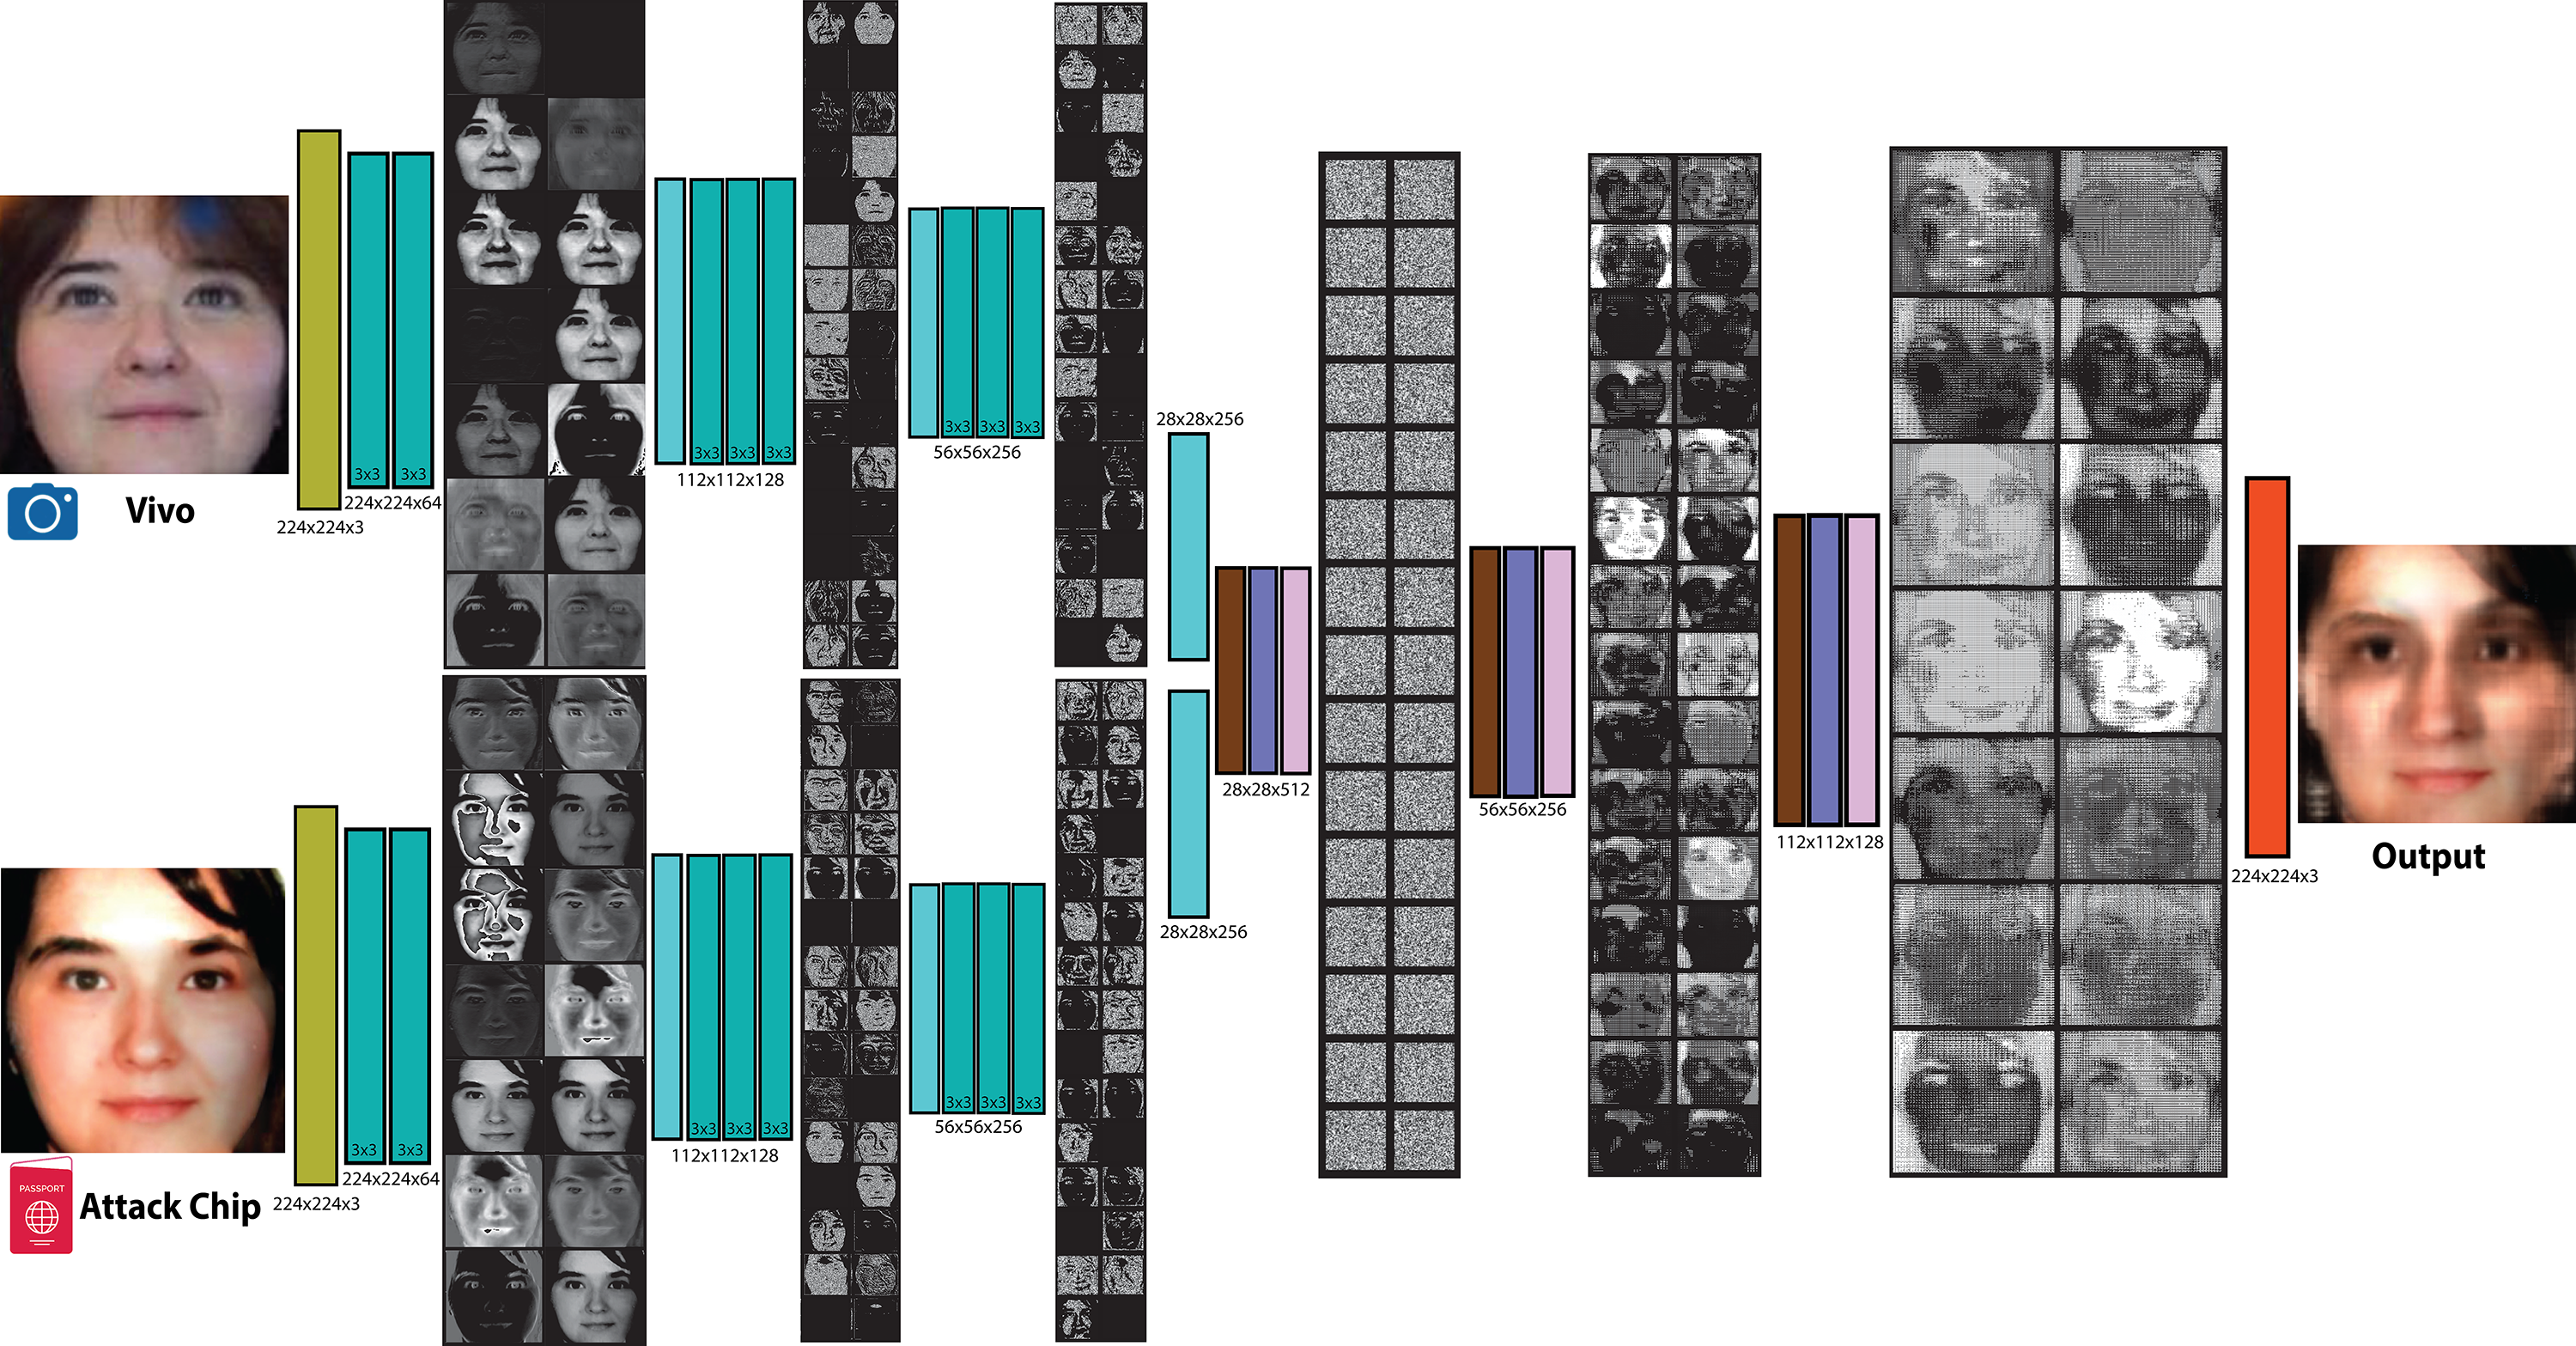
\includegraphics[width=1\textwidth]{ch-sistemasABC/images/ch-morphing/De-moprhingProcess.png}
    \caption{\textit{Resultado capas intermedias de \GLS{DMN}.}}
    \label{fig:MorphingAndDe-morphingExplanation}
\end{figure}

El proceso de \gls{de-morphing} se implementa mediante una \GLS{CNN} (ver Fig. \ref{fig:Arquitecturas} c)), con dos ramas de entrada que se encargan de la extracción de las características, una concatenación de estas características y una sucesión de capas de convolución transpuesta que reconstruyen la imagen discriminando las características que se encuentran en ambas imágenes. 

Las ramas de entrada copian su arquitectura del codificador de una arquitectura \gls{autoencoder} (ver Fig. \ref{fig:Arquitecturas} (b)) que a su vez copia las primeras capas de \Gls{VGG-Face} \cite{parkhi2015deep}, \cite{cao2018vggface2}, arquitectura especializada en reconocimiento facial (ver Fig. \ref{fig:Arquitecturas} (a)). 

% VGGFace (Parkhi, Vedaldi, Zisserman, \& Andrew, 2015) tiene una arquitectura similar a la de FACENet que al ser entrenada específicamente con caras, consiguiendo una precisión de 98,95 con LFW (Labeled Faces in the Wild  (G.B.Huang, 2007)) y de 97.3 con YTF (YouTube Faces (Wolf, Hassner, \& Maoz, 2011)).


%%% AUTOENCODER
\subsection{\textit{Autoencoder}}  \label{ref:Autoencoderfaces}

\begin{figure}[t!]
    \centering
    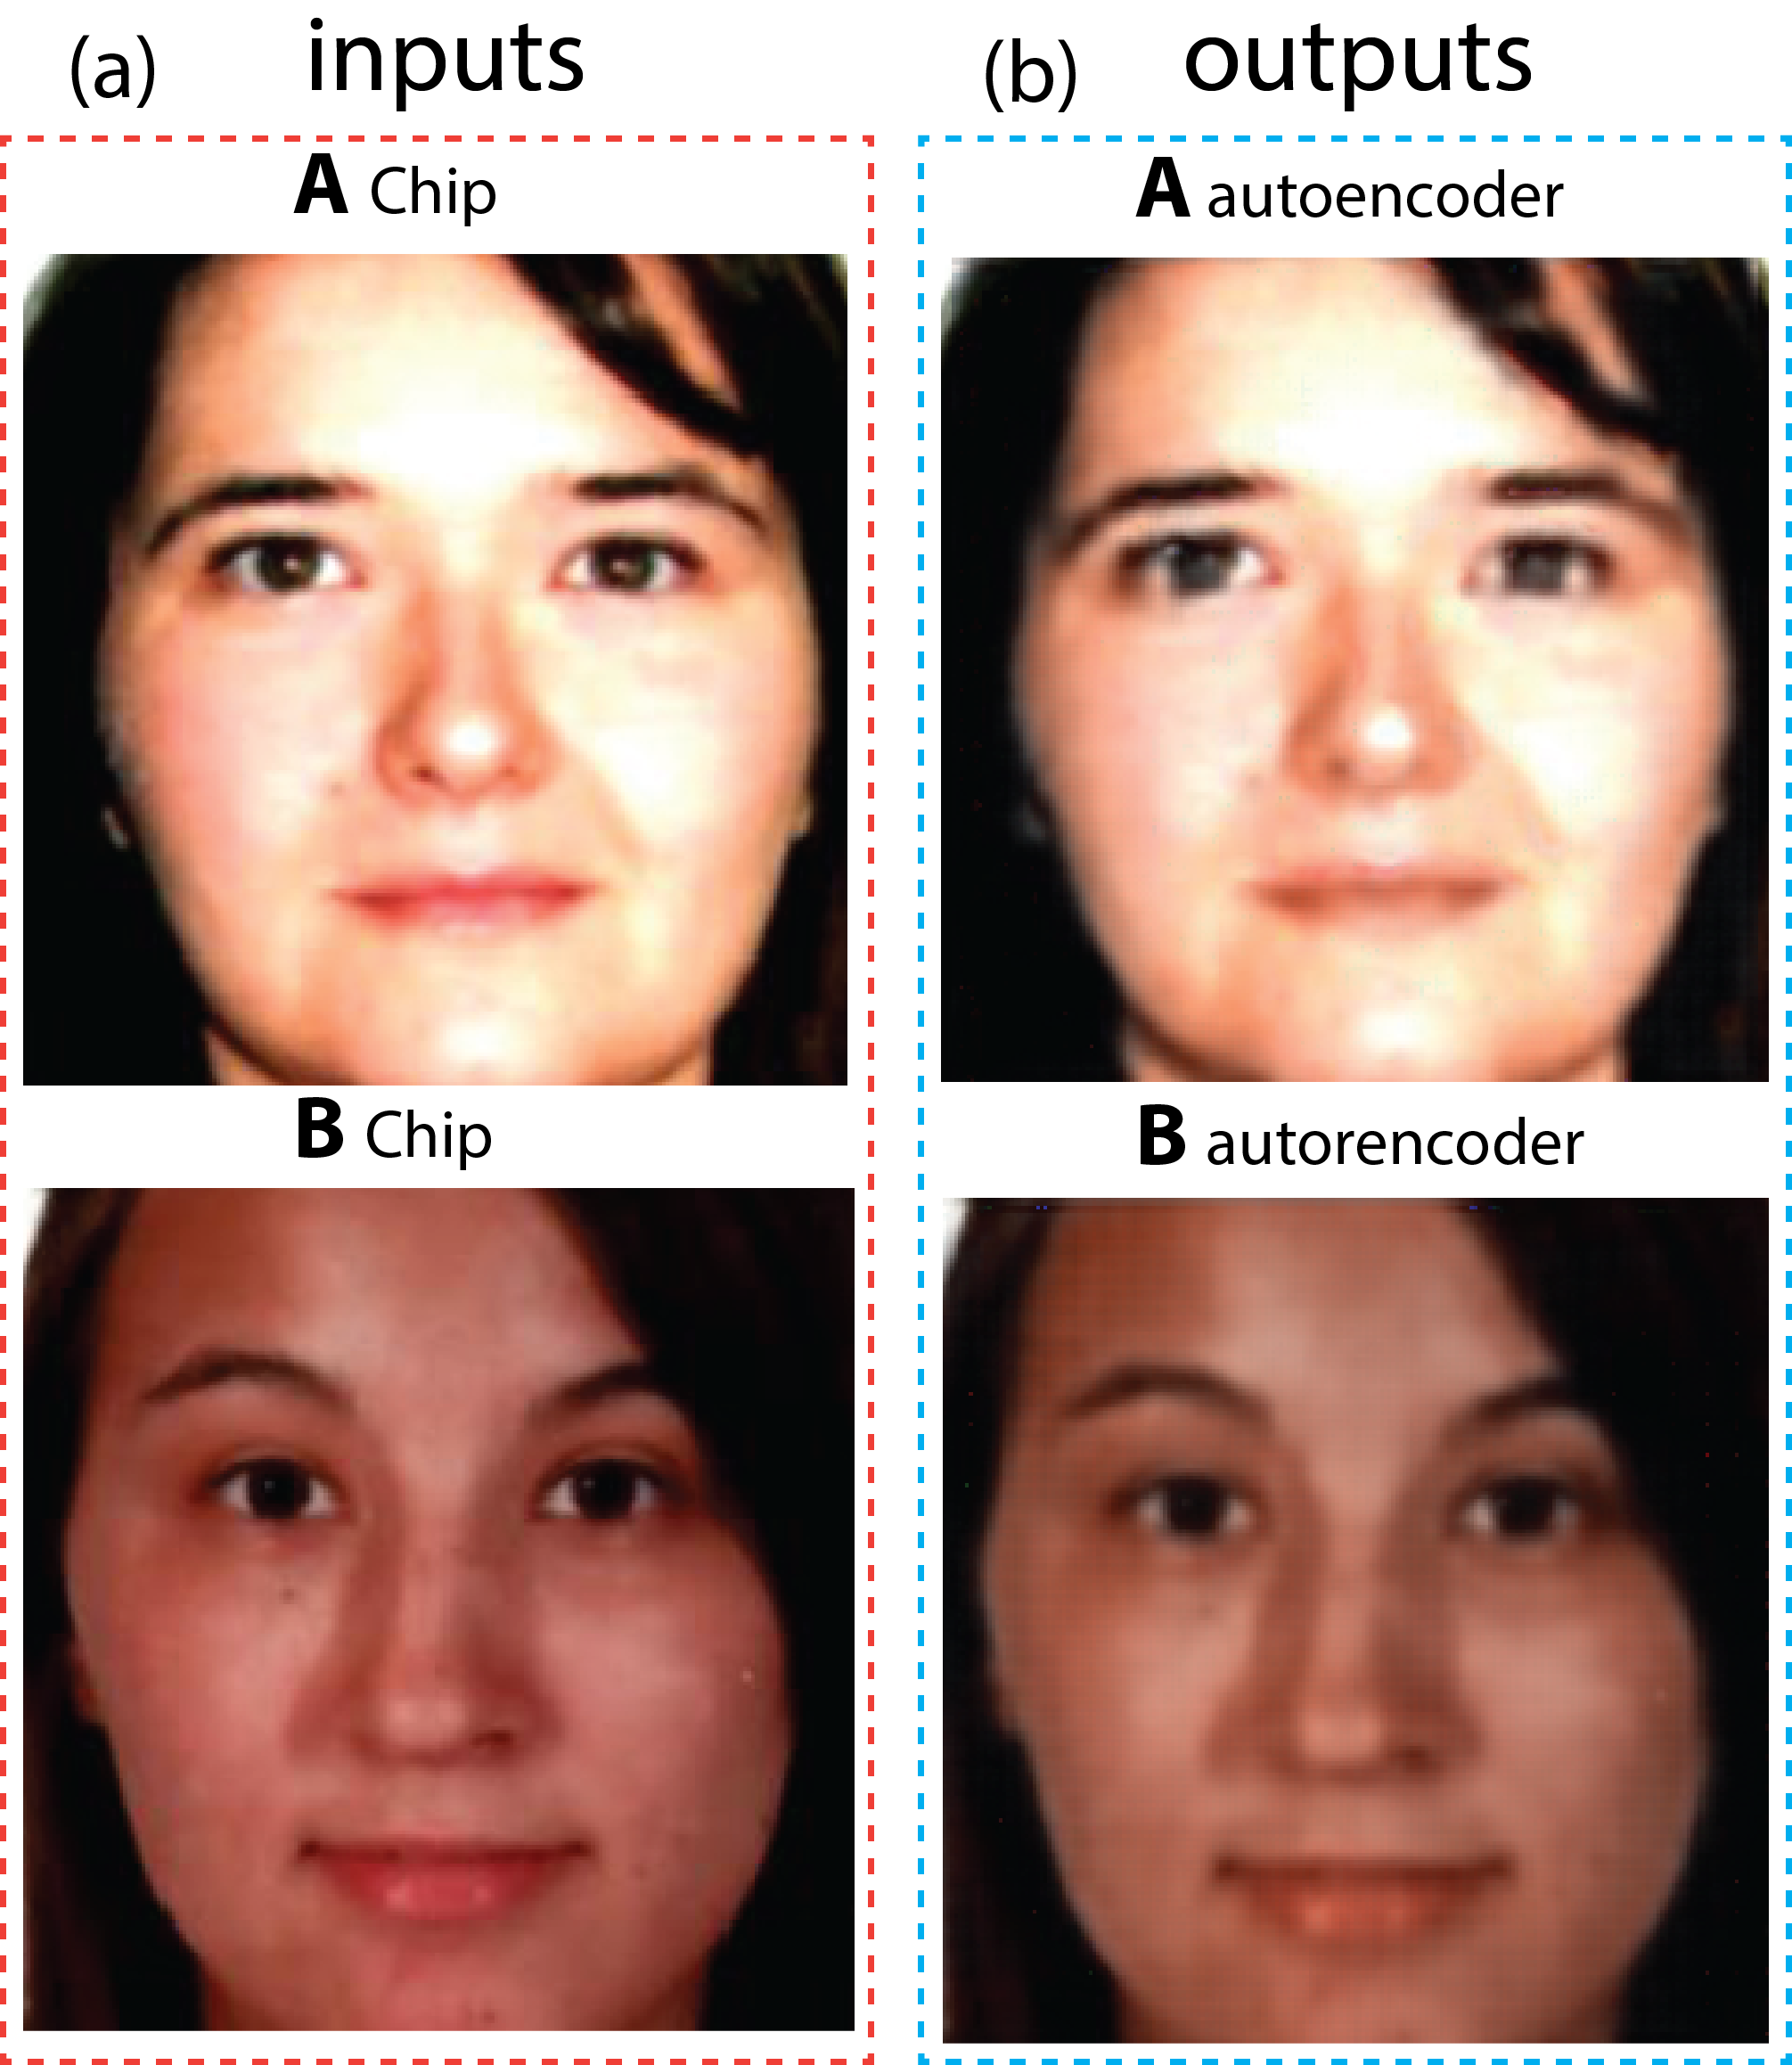
\includegraphics[width=0.5\textwidth]{ch-sistemasABC/images/ch-morphing/AUTOENCODER_CRISTINA_BEA.png}
    \caption{\textit{\Gls{autoencoder}} process with face image. \textit{\Gls{autoencoder}} process example: Original images (a) and Reconstructed images after \textit{\gls{autoencoder}} information extraction (b).}
    \label{fig:autoencoderImages}
\end{figure}

El \gls{autoencoder} (ver Fig. \ref{fig:Arquitecturas} (b)) tiene una arquitectura \GLS{CNN} similar a la descrita en \cite{deepLearningBook} que se divide en dos etapas: codificación y decodificación. Durante la codificación (línea discontinua azul), la imagen de entrada, de $224\times224\times3$ se reduce a un código o \textit{\gls{embedding}} de $28\times28\times256$, sin perder información descriptiva. En la decodificación (línea roja discontinua) se restaura la imagen de entrada partiendo del código usando una sucesión de capas de convolución transpuesta \cite{zeiler2010deconvolutional}. En la Fig. \ref{fig:autoencoderImages} con las imágenes de entrada (a) y de salida (b) del \gls{autoencoder}, se puede ver que las imágenes resultantes pierden algo de nitidez, pero conservan los rasgos que permiten una verificación facial.

La arquitectura del codificación en el \gls{autoencoder} es la idéntica a las capas iniciales de la red \Gls{VGG-Face} \cite{parkhi2015deep} (linea discontinua azul en Fig. \ref{fig:Arquitecturas} (a)), arquitectura \GLS{CNN} diseñada para la verificación facial, con altas tasas de precisión ($98.95\%$ con \textit{Labeled Faces in the Wild} (\GLS{LFW}) \cite{huang2008labeled} y $97.3\%$ con \textit{YouTube Faces} (\GLS{YTF}) \cite{wolf2011face}). Copiar la estructura de capas iniciales de \Gls{VGG-Face} garantiza una arquitectura adecuada para extraer información de imágenes faciales.

% Además de usar los pesos pre-entrenados de \textit{\Gls{VGG-Face}} para las capas de codificación, el autoencoder (codificador y decodificador) se entrenar para ajustar y optimizar los pesos atendiendo a las imágenes del problema actual.

La implementación del \gls{autoencoder} se llevó a cabo con la biblioteca \textit{TensorFlow Core v1.15} y se entrenó con imágenes de la base de datos \textit{CASIAWebFace} \cite{CASIAWebFace_DataBase}, utilizando de entrada y salida, en cada iteración, imágenes de una misma identidad con de $512$ muestras por \textit{batch}, durante $3000$ \textit{epochs} (exactamente $3206$ usando la opción \textit{<<early stopping>>} con valor de \textit{<<patience>>} de $500$ \textit{epochs}). Como función de perdida se uso \textit{Mean Squared Error} (\GLS{MSE}) y como algoritmo de optimización \textit{adaptive momentum} (\textit{Adam}) \cite{kingma2014adam} con una tasa de aprendizaje inicial de $0.005$ y disminuye a $0.001$. Respecto al \textit{hardware} se ha entrenado con una tarjeta gráfica \textit{NVIDIA GeForce GTX} $1050$ con $8$ GB RAM. 

% Por otra parte, es necesario evaluar la similitud entre las imágenes de entrada y de salida para comprobar el rendimiento del \textit{\gls{autoencoder}}. Para realizar esta evaluación, se procesaron imágenes \textit{chip} de $170$ dólares del corpus \Gls{FRAV-Morphing-Test} y se calcularon las probabilidades de aceptación del \textit{\gls{autoencoder}} y de la verificación facial \textit{\Gls{FaceNet}}. Además, se utilizó \textit{\Gls{FaceNet}} en lugar del corpus \textit{\gls{VGG-Face}} porque el primero evitaba los resultados ruidosos causados por el uso de la misma arquitectura de \textit{\gls{autoencoder}}.

%%% DEMORPHED NET
\subsection{DMN: \textit{Demorphing Network}} \label{ref:Decoderfaces}

Una vez que el proceso de codificación ha terminado, los dos \textit{\glspl{embedding} generados, de $28\times28\times256$, se concatenan en una única matriz de $28\times28\times512$}. Esta matriz contiene la información codificada de las imágenes de entrada. Y finalmente, mediante un decodificador que consiste en una sucesión de capas de convolución transpuestas, como se muestra en la Fig. \ref{fig:Arquitecturas} (c), se construye una imagen de salida con la misma resolución que las imágenes de entrada ($224\times224\times3$).

Para el entrenamiento se utilizaron $1000$ sujetos de \Gls{FRAV-Morphing-Test}: $700$ como conjunto de entrenamiento y $300$ como conjunto de validación. La repartición de los conjuntos se ha realizado a nivel sujeto para evitar el sobre-ajuste en el entrenamiento que se podría producir al mezclar identidades entre el entrenamiento y la validación.

Fusionado los \gls{chip} de los $1000$ sujetos de entrenamiento (todos con todos, menos cada uno consigo mismo) se consiguieron aproximadamente un millón de \gls{morphing} para entrenamiento. Como cada muestra de entrenamiento se compone de dos imágenes de entrada: el \gls{morphing} y el \gls{vivo} de una de las identidad, y el \gls{chip} de la otra identidad, como salida, realmente se entrenó con dos millones de muestras al poder alternar las identidades de dos sujetos por cada \gls{morphing}. 

Como el \gls{autoencoder}, \GLS{DMN} se implementó y entrenó con la biblioteca \textit{TensorFlow Core v1.15} durante $5000$ \textit{epochs}, con muestras de $512$ por \textit{batch}, con \textit{Mean Squared Error} (\GLS{MSE}) como función de perdida y \textit{adaptive momentum} (\textit{Adam}) \cite{kingma2014adam}  como algoritmo de optimización, con una tasa de aprendizaje inicial de $0.005$ y disminuye a $0.001$. Y en la misma tarjeta gráfica \textit{NVIDIA GeForce GTX} $1050$ con $8$ GB RAM. 

%%% RESULTADOS
\section{Resultados} \label{sec:morphingResultados}

\begin{figure}[t!]
    \centering
    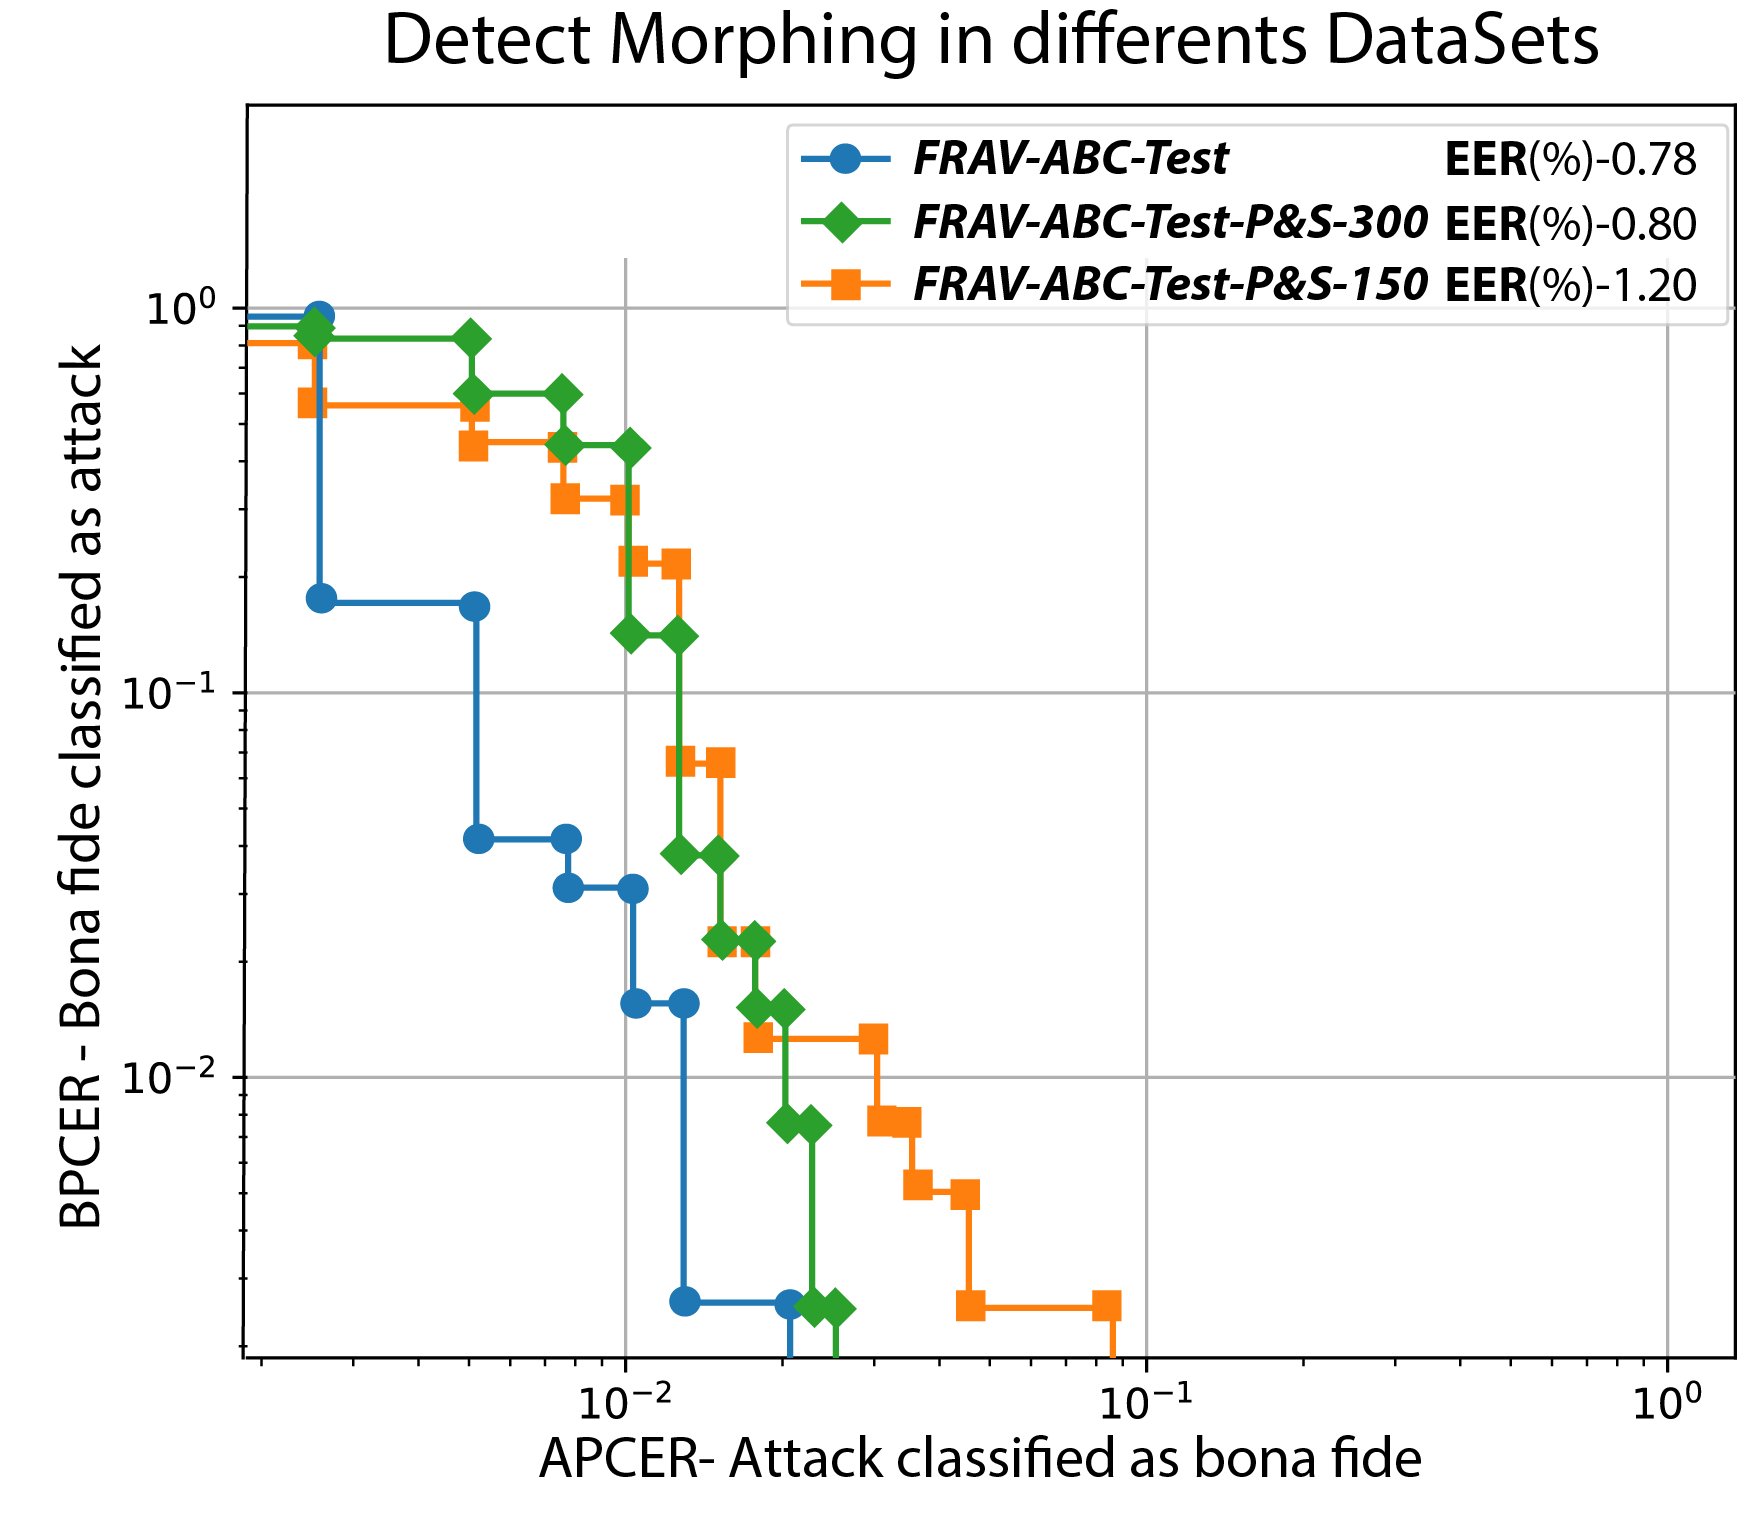
\includegraphics[width=0.6\textwidth]{ch-sistemasABC/images/ch-morphing/DEMORPHING_TEXT_PS300_PS150_CON_FORMAS.png}
    \caption{Curva de \GLS{DET} con \GLS{APCER} y \GLS{BPCER} con \Gls{FRAV-Morphing-Test}, \Gls{FRAV-Morphing-Test-PS-300} y \Gls{FRAV-Morphing-Test-PS-150}.}
    \label{fig:Morphingde-morphing}
\end{figure}

\begin{table}[t!]
\centering
\caption{Detección de \gls{morphing} en imágenes digitales y en imágenes impresas y escaneadas.}
\begin{tabular}{|c|c|c|c|c|}
\hline
\textbf{Tipo} & \textbf{Entorno} & \textbf{Enfoque} & \textbf{D-EER (\%)} & \textbf{ACC (\%)} \\ \hline
\multirow{4}{*}{Digital} & Lab & \cite{scherhag2017vulnerability} & 7.10 & - \\ \cline{2-5} 
 & Lab & \cite{raghavendra2017transferable} & 8.20 & - \\ \cline{2-5} 
 & Lab &  \cite{ferrara2019face} & 0.90 & 99.3 \\ \cline{2-5} 
 & ABC & DMN & \textbf{0.78} & \textbf{98.7} \\ \hline
\multirow{5}{*}{P\&S} & Lab & \cite{scherhag2017vulnerability} & 20.70 & - \\ \cline{2-5} 
 & Lab & \cite{raghavendra2017transferable} & 12.50 & - \\ \cline{2-5} 
 & Lab & \cite{ferrara2019face} & 6.10 & 93.5 \\ \cline{2-5} 
 & ABC (300dpi) & DMN & \textbf{0.80} & \textbf{98.2} \\ \cline{2-5} 
 & ABC (150dpi) & DMN & \textbf{1.20} & \textbf{98.1} \\ \hline
\end{tabular}\label{tab:comparative}
\end{table}

La Fig. \ref{fig:Morphingde-morphing} muestra las curvas \GLS{DET} de los errores \GLS{APCER} y \GLS{BPCER} obtenidos con \GLS{DMN} en las bases de datos: (\Gls{FRAV-Morphing-Test}, \Gls{FRAV-Morphing-Test-PS-300} y \Gls{FRAV-Morphing-Test-PS-150} (para  más información de estas bases de datos ver Sección \ref{sec:BBDD_Morphing}). La precisión del sistemas en la detección de ataques de \gls{morphing} es mayor del $98$\% con todas las bases datos y el \GLS{D-EER} no supera en ningún caso el $1.2$\%. 
 
En \Gls{FRAV-Morphing-Test} con imágenes digitales se obtiene un \GLS{D-EER} de $0,78$ y una precisión del $98,7$\% en la detección de ataques. En las otras bases de datos \Gls{FRAV-Morphing-Test-PS-300} y \Gls{FRAV-Morphing-Test-PS-150}, con imágenes impresas y escaneadas se obtienen resultados análogos. En \Gls{FRAV-Morphing-Test-PS-300}, un \GLS{D-EER} de $0,80$ y una precisión del $98,2$\%. Y en \Gls{FRAV-Morphing-Test-PS-150} un $1,20$ de \GLS{D-EER} de y un $98,1$\% de precisión.

Los mejores resultados se obtienen usando imágenes digitales pero lo más destacable, dado que es el procedimiento seguido por las autoridades de expedición de pasaportes, es que los resultados se mantienen con imágenes impresas y escaneadas tanto a una resolución de $150$ y como de $300$ \gls{DPI}, no apreciándose que exista una influencia significativa de la resolución del escaneo en los resultados de la detección. 

La Tabla \ref{tab:comparative} muestra una comparativa entre \GLS{DMN} y algunos de los enfoques \GLS{MAD} con mejores tasas de detección en el estado de arte. Se compara tanto el \GLS{D-EER} como la precisión, con imágenes digitales y con imágenes impresas y escaneadas. A la tabla también se han añadido las condiciones de adquisición de los datos procesados. Los resultados de este trabajo son los únicos que se han adquirido en las condiciones reales de un sistema \GLS{ABC}, el resto usan datos capturados en las condiciones controladas de laboratorio. 

Los resultados de \GLS{DMN} son mejores que los obtenidos con cualquiera de los estudios presentados. El \GLS{D-EER} con imágenes digitales es $14$\% inferior al mejor resultado logrado en la literatura y un orden de magnitud mejor que los otros.Y en el caso de las imágenes impresas y escaneadas el \GLS{D-EER} es un orden de magnitud mejor que todos los demás, tanto a $300$ como a $150$ \gls{DPI}.

El tiempo medio de ejecución del proceso de completo de detección es de $4,532$ segundos: $3.726$ el proceso del \GLS{DMN} y $0.403$ para cada una de las verificaciones (\gls{de-morphing} vs \gls{vivo} y \gls{de-morphing} vs \gls{chip}). Estos tiempos se han calculado con imágenes de prueba en un ordenador personal estándar sin requisitos especiales: Placa madre \textit{Intel \textregistered Core \texttrademark i$7$} con $8$ GB de RAM. Con lo que se cumplen ampliamente los requisitos mínimos de \Gls{frontex} que recomienda un tiempo inferior a $30$ segundos \cite{FRONTEX2016TechReport}.

%%% CONCLUSIONES
\section{Conclusiones} \label{sec:MorphingConclusiones}

En este capitulo se propone un nuevo enfoque de \GLS{MAD} para sistemas \GLS{ABC}, basado en \gls{de-morphing} e implementado con una \GLS{CNN} cuya arquitectura se compone de dos ramas de codificación y una de decodificación. El sistema ha sido entrenado y puesto a prueba con imágenes \gls{vivo} y \gls{chip} de un sistema \GLS{ABC} en un entorno real.

Se ha llevado a cabo una evaluación profunda del sistema propuesto y se ha comparado con tres estudios diferentes. obteniendo unos resultados con los que se puede concluir que el sistema resulta adecuado para detección de ataques. Cave destacar especialmente que los resultados obtenidos con imágenes impresas y escaneadas resultan notablemente mejores que los demás trabajos de investigación mencionados, siendo este el procedimiento que habitualmente se lleva a cabo en la expedición de pasaportes. 

Otro aspecto que distingue positivamente el enfoque propuesto es la posibilidad de extraer la identidad oculta del impostor o del cómplice lo podría ser de utilidad para otras aplicaciones. En futuros trabajos se hará hincapié en la mejora de calidad en la apariencia de las imágenes resultantes del proceso.

También en el futuro, se prevé aumentar el número de sujetos de las bases de datos, lo que permitirá un entrenamiento más intensivo del sistema para obtener mejores resultados y un mayor rendimiento.



